%\documentclass[12pt,preprint]{aastex}
\documentclass[]{spie}  
\renewcommand{\baselinestretch}{1.0} % Change to 1.65 for double spacing
\usepackage{amsmath,amsfonts,amssymb}
\usepackage{graphicx}
\usepackage[colorlinks=true, allcolors=blue]{hyperref}
\usepackage{url}
%\usepackage{natbib}
%\usepackage{xspace}
\def\arcsec{$^{\prime\prime}$}
\newcommand\degree{{^\circ}}
\newcommand\surfb{$\mathrm{mag}/\square$\arcsec}
\newcommand\Gyr{\rm{~Gyr}}
\newcommand\msun{\rm{M}_\odot}
\newcommand\kms{km s$^{-1}$}
\newcommand\al{$\alpha$}
\newcommand\ha{$\rm{H}\alpha$}
\newcommand\hb{$\rm{H}\beta$}
% from http://cdsads.u-strasbg.fr/abs_doc/aas_macros.html
\newcommand\aap{Astronomy and Astrophysics}
\newcommand\pasp{Publications of the ASP}
\newcommand\apjl{Astrophysical Journal, Letters}

 \newcommand{\arxiv}[1]{\href{http://arxiv.org/abs/#1}{arXiv:#1}}

\title{An Optical to IR Sky Brightness Model For the LSST}
\author[a]{Peter~Yoachim}
\author[b]{Michael~Coughlin}
\author[c]{George~Z.~Angeli }
\author[c]{Charles~F.~Claver }
\author[a]{Andrew~J.~Connolly}
\author[d]{Kem~Cook}
\author[a]{Scott~Daniel}
\author[a]{\v{Z}eljko~Ivezi\'{c}}
\author[a]{R.~Lynne~Jones}
\author[c]{Catherine~Petry}
\author[c]{Michael~Reuter}
\author[b]{Christopher~Stubbs}
\author[c]{Bo~Xin}

\affil[a]{University of Washington, Seattle, WA, USA}
\affil[b]{Harvard University, Boston, MA, USA}
\affil[c]{LSST Observatory, Tucson, AZ, USA}
\affil[d]{Cook Astronomical Consulting, CA, USA}


\authorinfo{Further author information:\\Peter Yoachim: E-mail: yoachim@uw.edu}

\pagestyle{empty}

\begin{document}

\maketitle

\begin{abstract}
  To optimize the observing strategy of the LSST, we require an accurate model of the night sky emission spectrum across a range of atmospheric conditions and from the near-UV to the near-IR.  We have used the ESO SkyCalc Sky Model Calculator \cite{Noll12,Jones13} to construct a library of template spectra for the Chilean night sky.  The ESO model includes emission from the upper and lower atmosphere, scattered starlight, scattered moonlight, and zodiacal light.
  We have then extended the ESO templates with an empirical fit to the twilight sky emission as measured by a Canon all-sky camera installed at the LSST site.

  With the ESO templates and our twilight model we can quickly interpolate to any arbitrary sky position and date and return the full sky spectrum or surface brightness magnitudes in the LSST filter system. Comparing our model to all-sky observations, we find typical residual RMS values of $\pm$0.2-0.3 magnitudes per square arcsecond.
\end{abstract}
\keywords{Astronomy Software, Python, Sky Emission}


\section{Introduction}

An accurate model of the background sky emission is needed to accurately simulate and schedule observations for the Large Synoptic Survey Telescope (LSST)\cite{Kahn16}.  To start building a complete sky emission model, we use the ESO SkyCalc Sky Model Calculator\footnote{\url{http://www.eso.org/observing/etc/bin/gen/form?} \url{INS.MODE=swspectr+INS.NAME=SKYCALC}} \cite{Noll12,Jones13}.  The ESO model includes scattered moonlight, scattered starlight, zodiacal light, molecular emission from the lower atmosphere, emission lines from the upper atmosphere, and airglow continuum.  The ESO model is designed for Cerro Paranal, which is very similar to Cerro Pachon.  Pachon is located 625 km south of Paranal, at an altitude of 2,700m compared to Paranal at 2,600m.  

The ESO model computes the expected sky background from different sources from first principles (e.g., single and double scattering of lunar light). Because LSST will want to compute the sky background for the full sky millions of times throughout the 10-year survey, we need to improve performance by pre-computing the ESO model on relevant parameter grids and interpolating the results to our specific observing conditions. Also, the ESO source code is not publicly available, limiting our ability to run it directly at scale.

Our new sky brightness code described in this paper can be found at \url{https://github.com/lsst/sims\_skybrightness}. In \S\ref{sec:eso} and~\ref{sec:interp}, we give a brief description of the sky components in the ESO model and how we interpolate their results. In \S\ref{sec:obs} and~\ref{sec:twi} we describe observations taken on Cerro Pachon and how we have used those observations to construct a model of the twilight sky brightness.  Finally, \S\ref{sec:validate} shows how we have validated the model.

\section{The ESO Model}\label{sec:eso}

In this section, we briefly describe the sky components included in the ESO model and how we have created grids of model spectra with them. The ESO model is described in detail in Ref.~\citenum{Noll12} and~\citenum{Jones13}.

For each ESO model component, we save the output spectra as \texttt{numpy} zip files.  The model spectra run from 300 nm to 2 microns, with 0.1 nm stepsize.  In addition to the spectra, we use the LSST filter response curves to pre-compute the 6 LSST magnitudes for each spectrum at each grid point. These $\sim$3,500 pre-computed spectra and $\sim$21,000 magnitudes are stored in their own git repository (\url{https://github.com/lsst/sims\_skybrightness\_data}) and total about 1 Gb in size. For all the models we use the average precipitable water vapor (2.5 mm), set the time of night to be the middle of the night, and the season to be the annual average.

\subsection{Zodiacal Light}

Zodiacal light is caused by sunlight scattered by dust grains in the plane of the ecliptic.  The ESO model varies the Zodiacal light as a function of ecliptic coordinates and airmass.  

We use an airmass grid of 1, 1.2, 1.4, 2.0, and 2.5 and a Healpixel\footnote{\url{http://healpix.sf.net}} \cite{Gorski99} grid with 192 elements (nside=4, resolution of $\sim15\degree$).  We use the ESO calculator to generate spectra at the center of each Healpixel coordinate and each airmass value, resulting in 960 zodiacal spectra that we can then interpolate to arbitrary position and airmass.  The Healpixels are a grid in heliocentric ecliptic latitude and longitude (i.e., longitude zero is fixed to the solar position).  Some example zodiacal light spectra are shown in Figure~\ref{fig:zodiacal}. 


\begin{figure}[ht]
  \begin{center}
  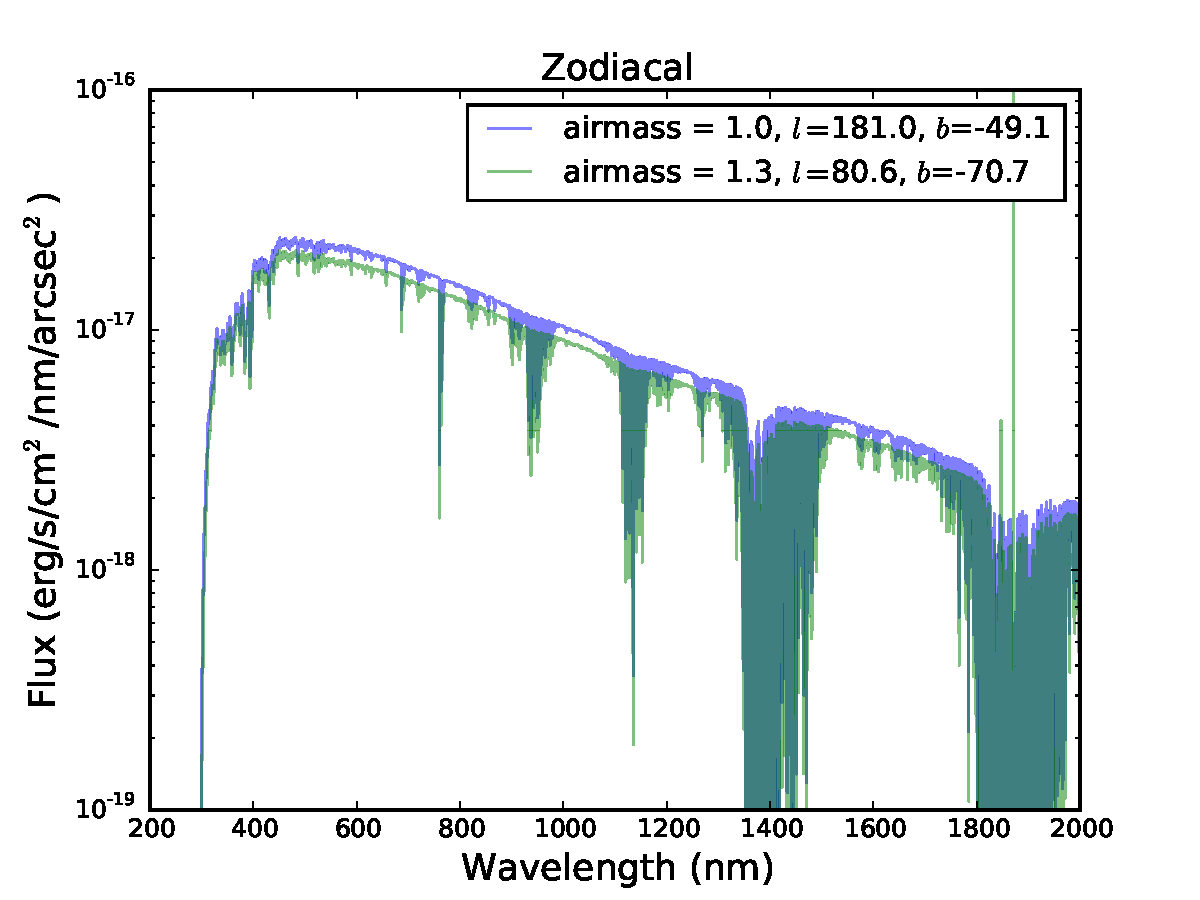
\includegraphics[height=7cm]{plots/zodiacal.pdf}
  \end{center}
  \caption{Example of zodiacal light interpolated from ESO templates. \label{fig:zodiacal}}
\end{figure}


\subsection{Scattered Moonlight}

Ref.~\citenum{Krisciunas91} provide one of the most popular models for computing the scattered moon light. This model is based on observed magnitudes from Mauna Kea. The ESO code uses the updated model of Ref.~\citenum{Jones13} which is fully spectroscopic and designed for Cerro Paranal. Ref.~\citenum{Jones13} claim their model uncertainty is $<20$\% in the optical.  Unlike the Ref.~\citenum{Krisciunas91} model that is a fit to observed broadband sky brightnesses, the Ref.~\citenum{Jones13} model uses fully 3D single scattering calculations and provides an entire spectrum. The Ref.~\citenum{Jones13} model does a better job matching observations than the Ref.~\citenum{Krisciunas91}, particularly at short wavelengths.

We build a template library of scattered moonlight by considering moon-sun separations of 0$\degree$\ to 180$\degree$ in 15 degree steps, and moon altitudes from 15$\degree$\ to 90$\degree$.  We then compute the expected spectrum on a grid of 29 positions across the sky. This is a Healpixel grid (with an nside of 4, resolution of $\sim15\degree$), based on altitude and azimuth (relative to the moon), where we ignore pointings with an airmass greater than 2.6. This results in a total of 2,262 template spectra for the scattered moonlight. Examples of the scattered moonlight spectra are shown in Figure~\ref{fig:moon}.

\begin{figure}[ht]
  \begin{center}
  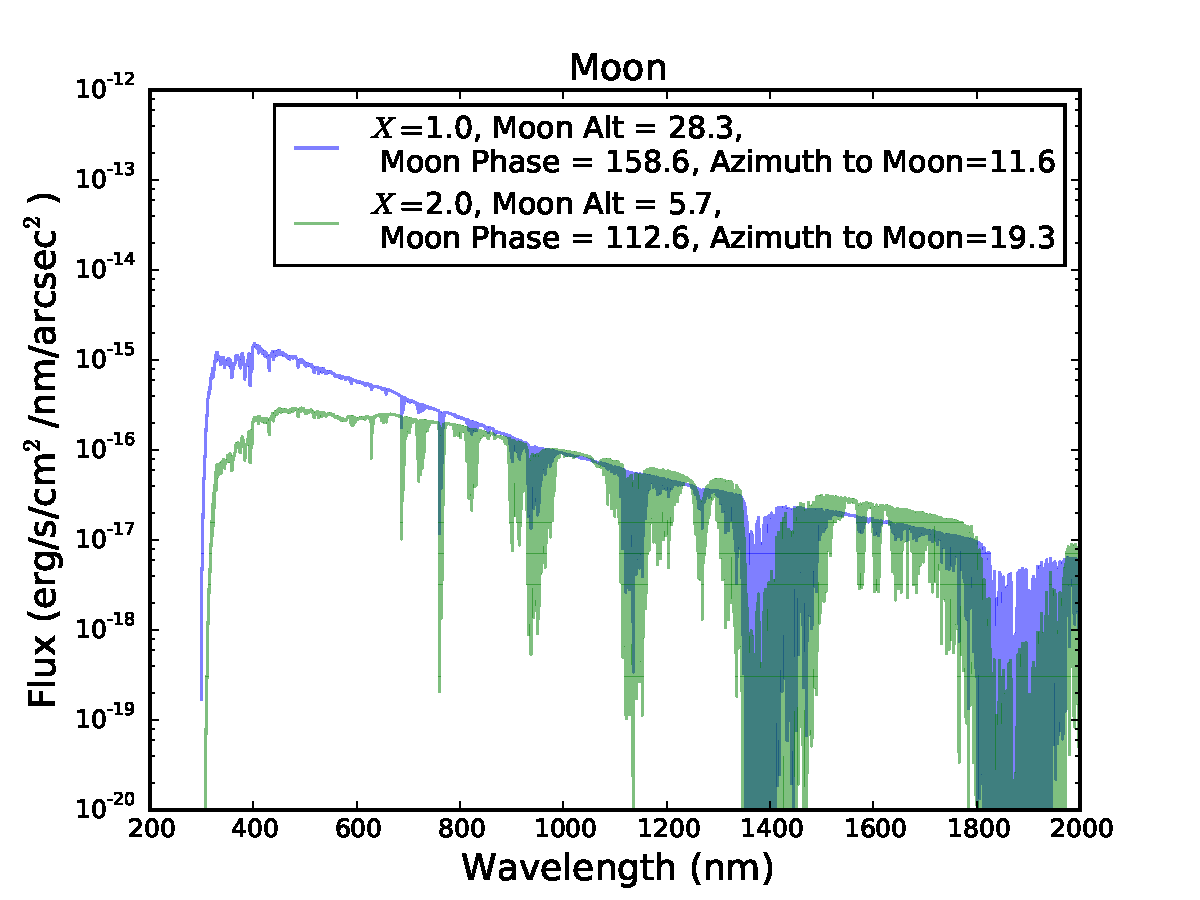
\includegraphics[height=7cm]{plots/moon.pdf}
  \end{center}
  \caption{Example of the scattered lunar light. \label{fig:moon}}
\end{figure}


\subsection{Airglow}

The airglow is assumed to be a function of airmass and solar activity as measured by solar radio observations.  We compute the spectra on a grid of airmass of 1 to 2 with steps of 0.1 and additionally an airmass of 2.5.  For the solar activity, we span 50 to 310 solar flux units (1 SFU = 4$0^4$ Jy) with a step size of 20, resulting in a total of 168 airglow spectra. 

Technically, the airglow also varies with the time of year and time of night. \citenum{Patat08} also shows the seasonal variation is negligible in $B$, and grows to around a peak amplitude of $\sim\pm0.25$ mags/sq arcsecond in $I$, which is similar to our overall RMS residuals. Examples of the airglow spectra are shown in Figure~\ref{fig:airglow}. 

\begin{figure}[ht]
\begin{center}
  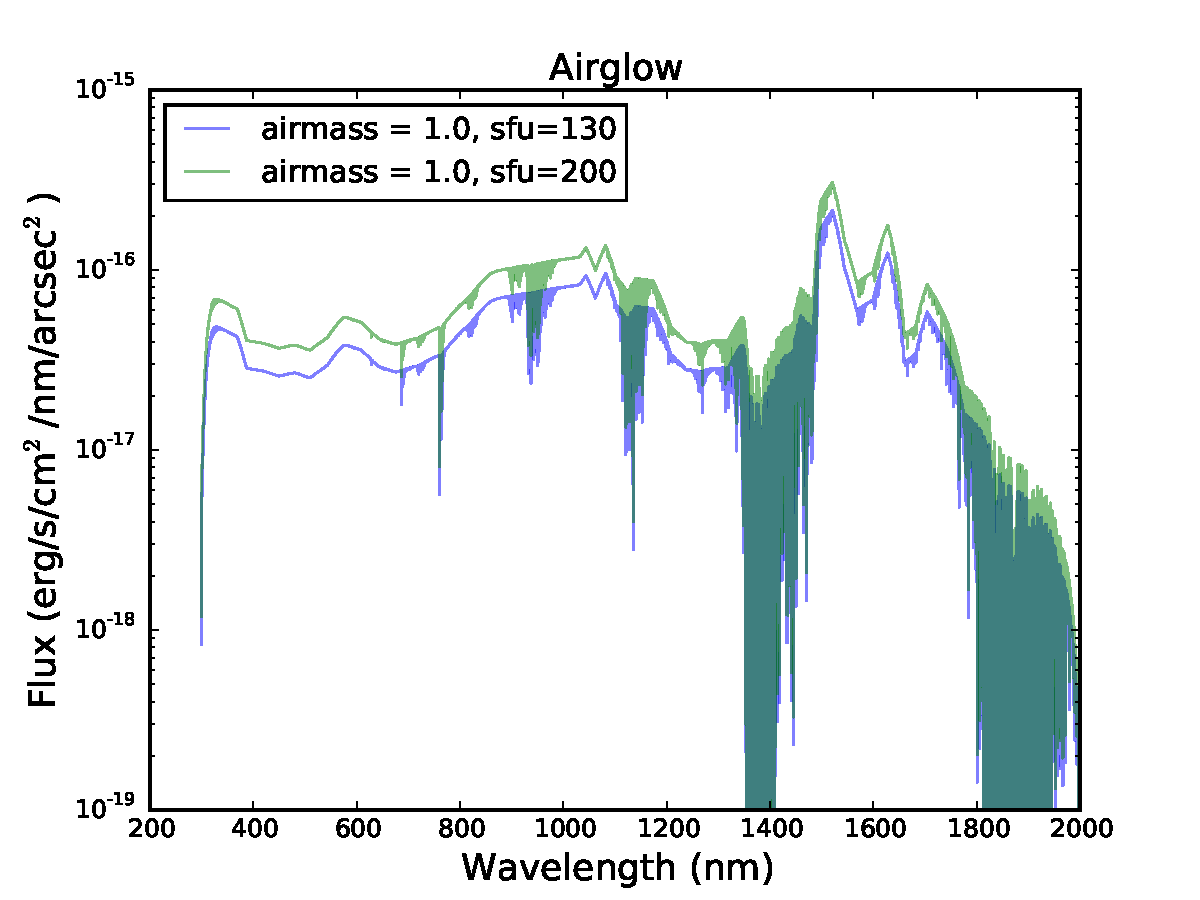
\includegraphics[height=7cm]{plots/airglow.pdf}
  \end{center}
  \caption{Example of airglow spectra. \label{fig:airglow}}
\end{figure}

  

\subsection{Scattered Star Light}

The scattered star light is a very minor component in the sky background, thus the ESO model uses a mean spectrum for the scattered starlight.  An example of the scattered star light is show in Figure~\ref{fig:merged}. This component in only a function of airmass.


\subsection{Atmospheric Emission Lines}

The airglow and emission lines vary through the night and by season, but Ref.~\citenum{Noll12} show the variation is at the 10-20\% level.  Since LSST is a broad band survey, such mild changes in narrow emission features should not strongly effect the integrated sky background.  For scheduling observations, the variation in background caused by airmass should swamp any effects from the skylines fading during the night.

The lower atmosphere only contains emission in the IR, but we have included it for completeness.  We assume the atmospheric emission is a function of only airmass and take template spectra at with airmass of 1 to 2 with steps of 0.1 and additionally an airmass of 2.5.

Because the upper atmosphere, lower atmosphere, and scattered star light only vary as a function of airmass, we have combined them into a single component in the code. Example of the spectra are shown in Figure~\ref{fig:merged}.


\begin{figure}[ht]
  \begin{center}
  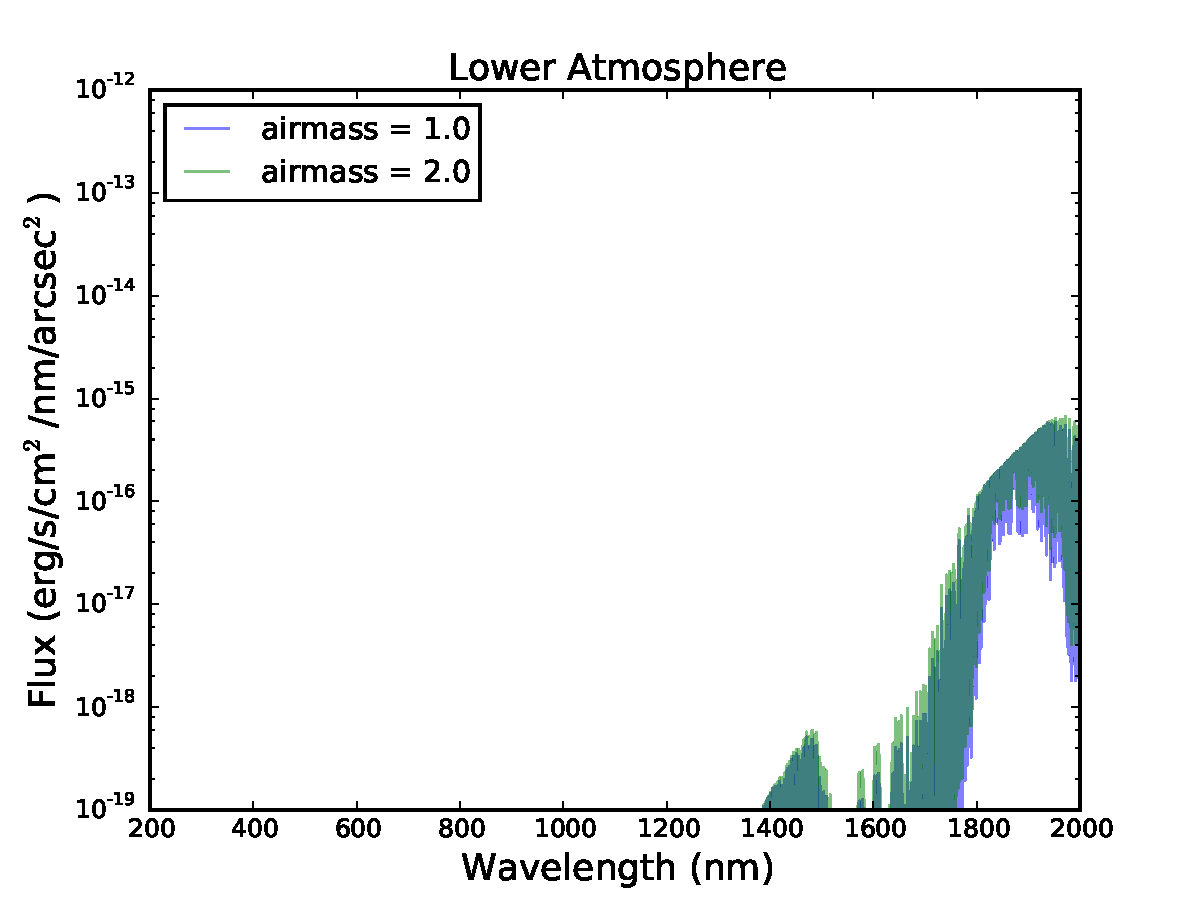
\includegraphics[height=5cm]{plots/merged0.pdf}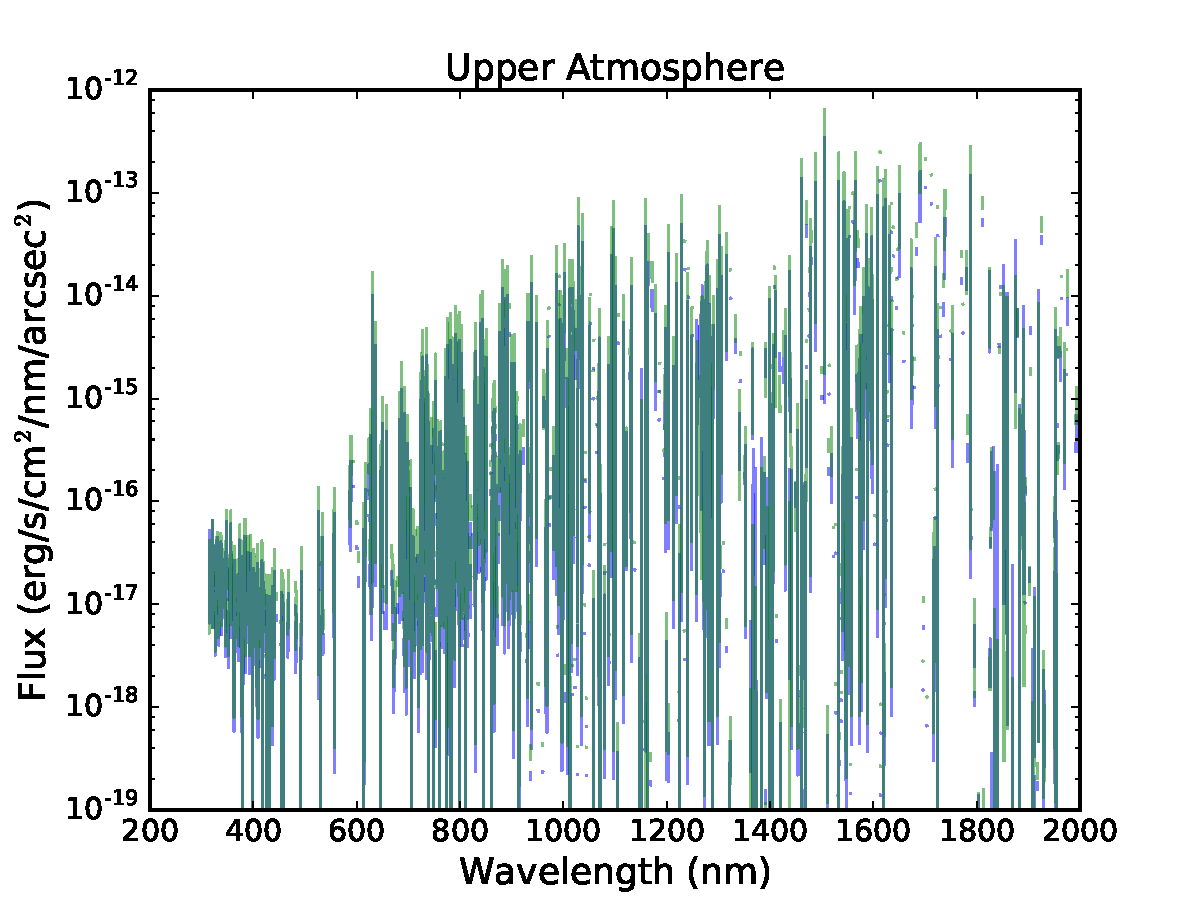
\includegraphics[height=5cm]{plots/merged1.pdf} \\
  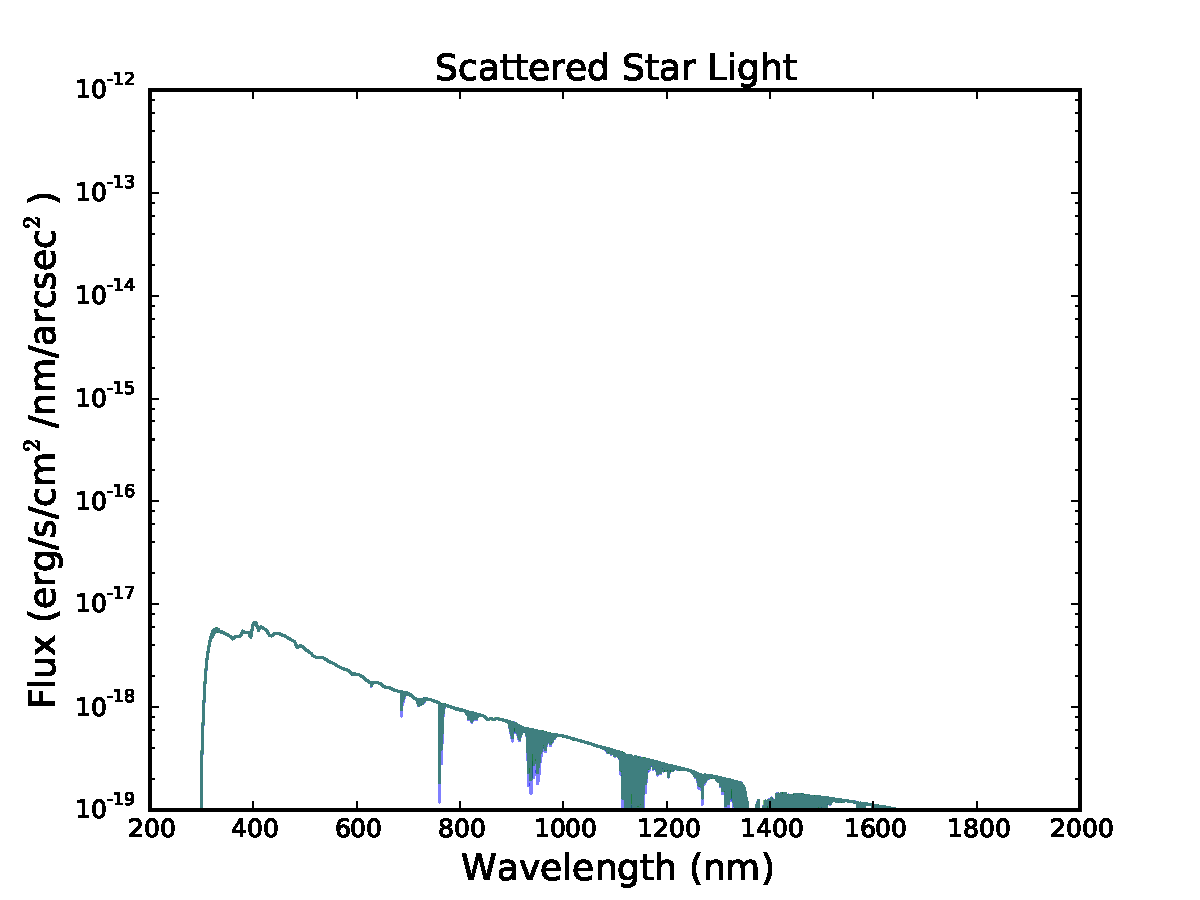
\includegraphics[height=5cm]{plots/merged2.pdf}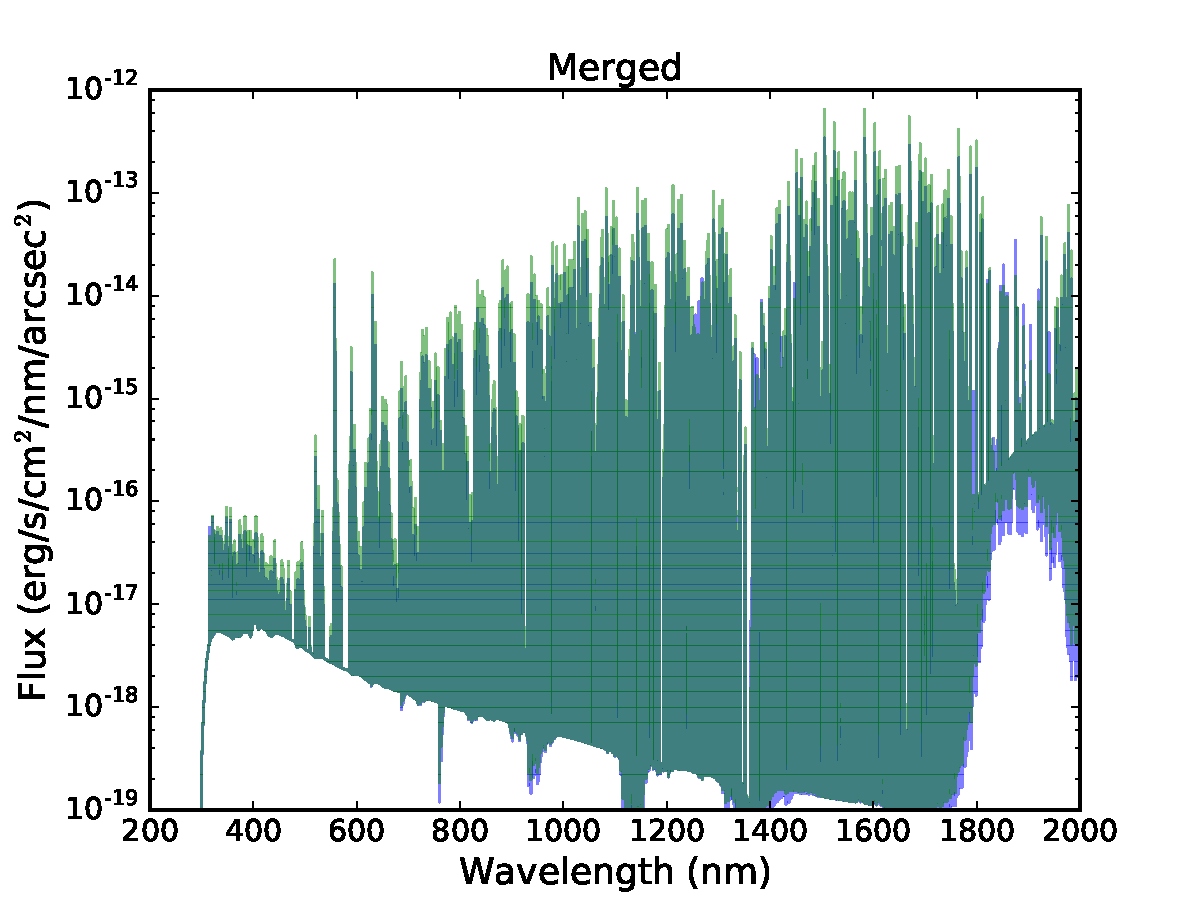
\includegraphics[height=5cm]{plots/merged3.pdf}
  \end{center}
  \caption{Examples of the sky brightness components that are only dependent on airmass. \label{fig:merged}}
\end{figure}


\section{Interpolating the Templates}\label{sec:interp}

For all the interpolations, we weight and average the base-10 logarithm of the template spectra (or average the magnitudes).  In the future, we could experiment with switching between interpolating the spectra and the log of the spectra based on how much variation there is between interpolation points.  We use linear interpolation (e.g., the spectrum of an observation at an airmass of 1.02 will be the sum of 0.8 times the airmass 1.0 template and 0.2 times the airmass 1.1 template). 

For the Zodiacal and Lunar components, since we have placed the templates at Healpix grid-points, we can use fast healpy\footnote{\url{https://github.com/healpy/healpy}} routines to find the 4 nearest Healpixel points, along with their weights.  


\section{Observations}\label{sec:obs}

Several sky monitoring instruments have been installed at the LSST site on Cerro Pachon.  In this paper, we use data from a Canon 5D Mark III digital SLR with a 15mm focal length f/2.8 Sigma fisheye lens, pointed at the zenith. The camera is installed beneath a hemispherical plexiglass dome that is installed in the roof of the ALO building on the Cerro Pachon ridge.  The CMOS imager in the Canon 5D camera has a Bayer array in the focal plane, with sub-pixels allocated to BGGR.  These bands are fairly close to the astronomical standard BVR set of filters. Although one can obtain modified Canon cameras with the NIR-blocking filter removed, the unit we installed in Jan 2014 was an off-the-shelf version. This means the sky brightness in these bands will be dominated by scattered and reflected sunlight and unresolved sources, but we aren't sensitive to OH emission.  This setup has been taking data since Jan 2014.  The Canon takes 30 second exposures in RGB filters throughout the night and during twilight. 

The current analysis pipeline for the Canon data takes aperture photometry of bright stars and records their magnitudes as well as the sky brightness measured in an annulus around each star.  We have combined the observations into a database from 42,000 images producing 91.5 million photometric measurements spanning 311 days.  A seperate reduction pipeline to analyze the distribution of clouds from the same observations is described in Ref.~\citenum{Yoachim16}.

We use these sky observations to fit a twilight sky brightness model and verify the other components of the sky brightness model.

\section{Additional Components}\label{sec:twi}
\subsection{Twilight}

The ESO sky model does not include a component for sunlight scattered by earth's atmosphere.  The twilight sky brightness is difficult to compute analytically.  While scattered moonlight can be computed via a single or double scattering model, the solar twilight comes from multiple scatterings, thus there is no simple analytic model for computing the solar twilight from first principles and models must instead rely on Monte Carlo radiative transfer simulations \cite{Patat06}.

Rather than compute radiative transfer, we fit a simple empirical model to the twilight flux.  Data from the all-sky camera as well as other sites show that after the sun's altitude drops below $\sim-10\degree$ the twilight flux decays exponentially with solar altitude. The total sky brightness is well fit by an exponential decay plus a constant floor.  In Figures~\ref{fig:twiSky} and~\ref{fig:twiExp} we show that when one uses alt-az coordinates, where azimuth is heliocentric (sun always at an azimuth of zero), the twilight is well described as an exponential decay plus a constant for all points in the sky.  %Figure~\ref{fig:compareZenithCanon} shows that the Canon all-sky camera does see the expected sharp transition at moonrise.  



% from twiPlotsForDoc.py
\begin{figure*}[ht]
  \begin{center}
  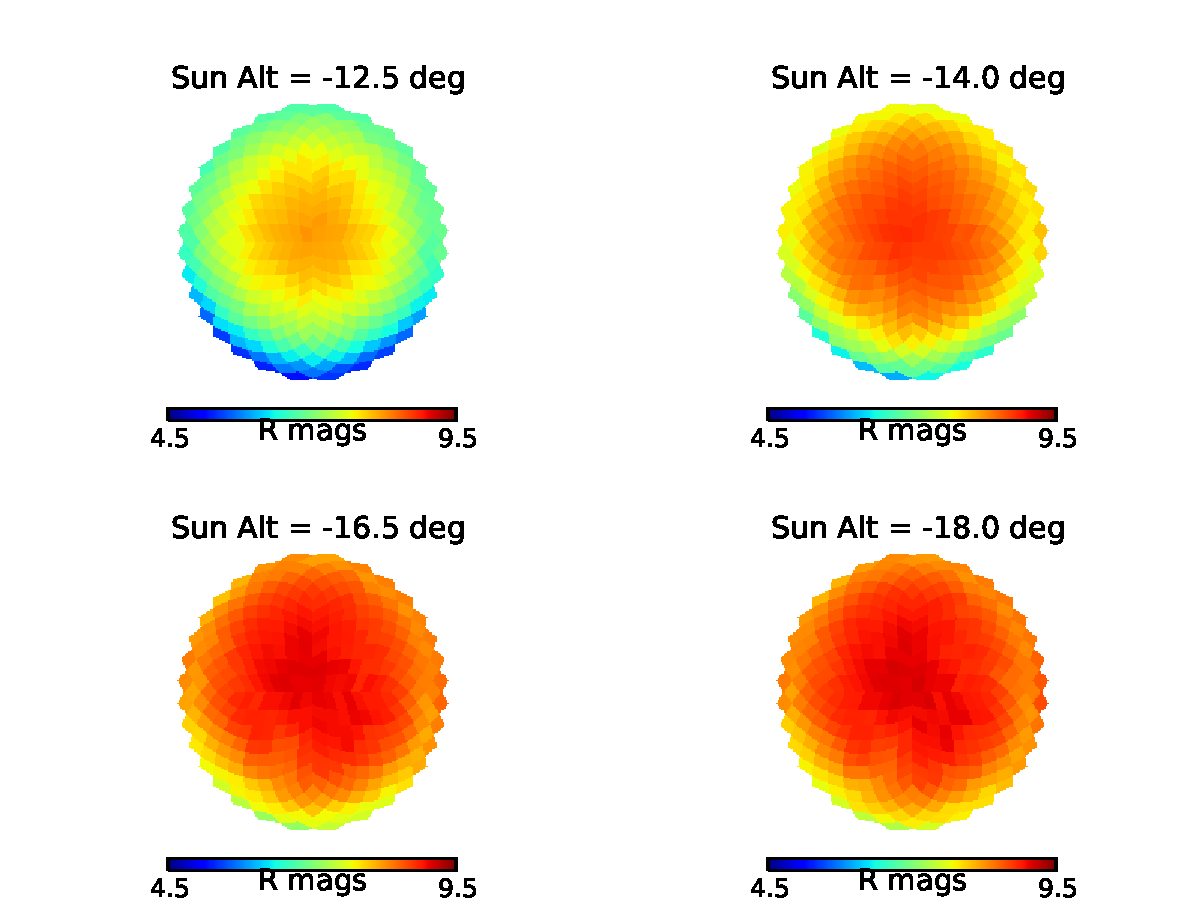
\includegraphics[height=7cm]{plots/twiExamples.pdf}
  \end{center}
  \caption{Sky brightness values measured from the Canon all-sky camera after median binning spatially by Healpixels and combining similar sun altitude observations. Only frames with the moon below the horizon were used. Zenith is at the center of each image, and the sun is below the horizon at an azimuth of zero (bottom of the frame). The values are instrumental magnitudes.  \label{fig:twiSky}}
\end{figure*}


% from fitTwiSlopesSimul.py
\begin{figure*}[ht]
  \begin{center}
  \begin{tabular}{c c}
  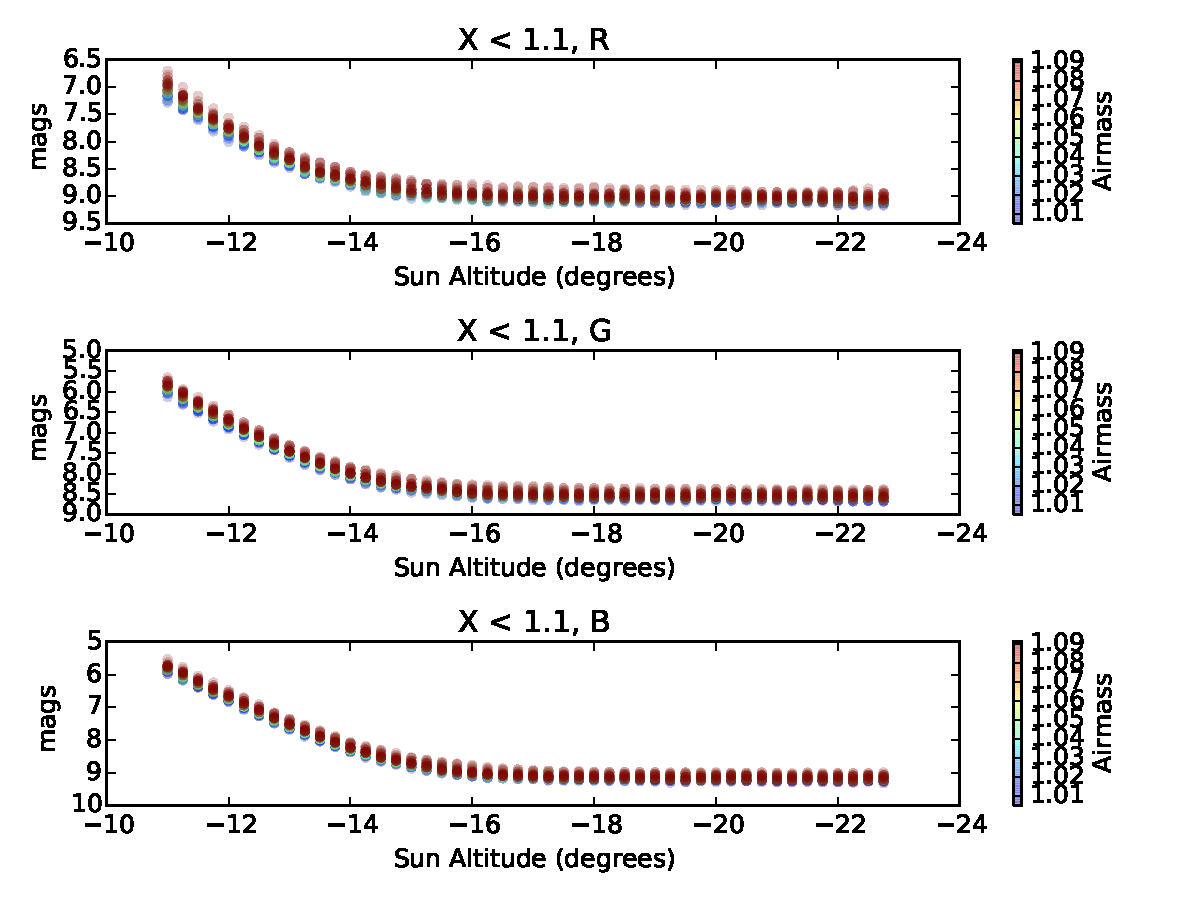
\includegraphics[height=7cm]{plots/altDecay.pdf} & 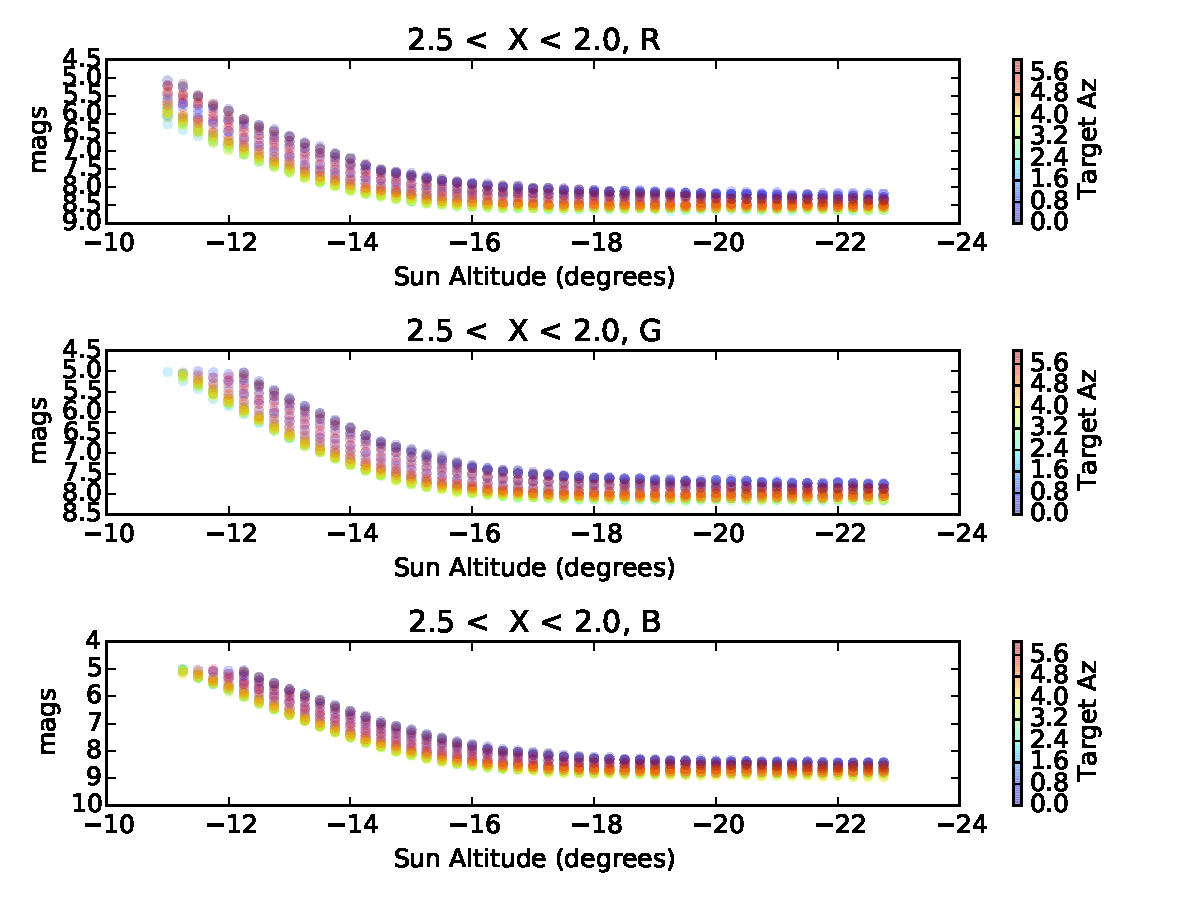
\includegraphics[height=7cm]{plots/altDecayHA.pdf}
  \end{tabular}
  \end{center}
  \caption{Photometry from the Canon all-sky camera, after it was been median-binned and selected for only times where the moon is down.  At low airmass (left panels), the sky brightness decays exponentially and has a small variation that is dominated by the change in airmass.  At higher airmasses (right panels), the decay is still exponential, but now is a function of both airmass and azimuth relative to the sun. \label{fig:twiExp}}
\end{figure*}



To model the broadband flux from only the scattered twilight, we first model the flux from scattered sunlight in the hemisphere pointed away from the sun as
\begin{equation}\label{eqn:twi1}
  f^{away} = f_{z} r_{12/z} 10^{a(\alpha+12^{\circ})+b(X-1)}
\end{equation}
where $\alpha$ is the altitude of the sun, $X$ is the airmass, $f_{z}$ is the flux at zenith during dark-time, and $r_{12/z}$ is the ratio of the 12-degree twilight zenith flux to the dark-time zenith flux. The full twilight flux in any direction is then given by
\begin{equation}
  \label{eqn:twi}
  f^{twi}  = \left\{
  \begin{array}{@{}ll@{}}
        f^{away}, & \text{if}\  \pi/2 < \phi < -\pi/2  \text{ or } X < 1.1\\
        f^{away} 10^{c (X-1) \cos{\phi}}, &  \text{if}\   \pi/2 > \phi >  -\pi/2 \text{ and } X > 1.1
        \end{array} \right.
\end{equation}
where $\phi$ is the azimuthal angle relative to the sun. The total sky background flux at zenith is then given by $f = f^{twi} + f_{z}$. Equation~\ref{eqn:twi} can be converted to magnitudes by:
\begin{eqnarray}
  m^{away} = m_0 -2.5a(\alpha+12^{\circ})-2.5b(X-1) \\
  m^{toward} = m^{away} -2.5c(X-1)\cos{\phi}
\end{eqnarray}
where $m_0$ is the scattered sunlight component to the 12-degree twilight surface brightness at zenith.  

By default, we only apply the twilight component for solar altitudes between -11 and -20 degrees. For solar altitude values less than -20 degrees, we find the other sky components always dominate. For altitudes greater than -11, our simple model breaks down but we expect LSST exposures would saturate well before this level.  

We have taken the sky brightness measurements from the Canon camera (when the moon is down) and median-binned the data based on sun altitude and alt-az coordinate.  The median binning effectively eliminates cloudy data.  Some example R-band twilight maps are shown in Figures~\ref{fig:twiSky} and~\ref{fig:twiExp}.  We use these data to find the best-fitting parameters for Equation~\ref{eqn:twi}.  

The best fitting parameters for $r_{12/z}$, $a$, $b$, and $c$ for each of the Canon filters as well as fits from the literature are listed in Table~\ref{table:canonFits}.  One important lesson from the data is the counter-intuitive result that during twilight the darkest part of the sky is near zenith, not moderate airmass in the hemisphere facing away from the sun. One is much better off observing at low airmass towards the sun rather than high airmass away from the sun.

%>>> import lsst.sims.skybrightness as sb
%>>> twi = sb.TwilightInterp()
%>>> twi.printFitsUsed()
\begin{table}
\caption{Final parameters for equation~\ref{eqn:twi} used by the sky brightness twilight component. 
\label{table:canonFits}}
\begin{center}
\begin{tabular}{c c c c c c c}
  Filter & $r_{12/z}$ & $a$  & $b$  & $c$  & $f_z,dark$ & m$_z,dark$ \\
  & & (1/radians) & (1/airmass) & (az term/airmass) & (erg/s/cm$^2$)$\times 10^8$ \\
  \hline
  \hline
  B  & 8.42 & 22.96 & 0.29 & 0.30 & 3.05  &  22.35 \\
  G  & 4.14 & 22.94 & 0.30 & 0.32 & 5.50  &  21.71 \\
  R  & 2.73 & 22.20 & 0.30 & 0.33 & 8.02  &  21.30 \\
  $z^{\rm{a}}$ & 2.29 & 24.08 & 0.30 & 0.30 & 50.58  &  19.30 \\
  $y^{\rm{a}}$  & 2.0 & 24.08 & 0.30 & 0.30 & 167.50  &  18.00 \\
  $u^{\rm{b}}$  & 16.00 & 22.96 & 0.29 & 0.30 & 2.01  &  22.80\\
 \hline
 \multicolumn{7}{l}{$^{\rm{a}}$The $z$ and $y$ fits are based on $I$-band fits from \cite{Patat06}.} \\
 \multicolumn{7}{l}{The $b$ and $c$ terms are assumed to be similar to the other optical filters.} \\
 \multicolumn{7}{l}{$^{\rm{b}}$The $u$ filter is assumed to be identical to $B$, but with a brighter $r_{12/z}$ value.}
 \end{tabular}
 \end{center}
\end{table}


While the parameters in Table~\ref{table:canonFits} do a reasonable job reproducing the observed magnitudes, we are also interested in generating the full spectrum of the sky.  For this, we assume the twilight is a modified solar spectrum.  We multiply a solar spectrum\footnote{\url{http://rredc.nrel.gov/solar/spectra/am0/ASTM2000.html}} by a low order polynomial such that it reproduces the expected broad band magnitudes.  One obvious shortcoming of this approach is that we have not included the effects of atmospheric transmission on the twilight sky spectrum. We could upgrade the code by using a library of twilight spectra scaled to the correct magnitudes, however, few spectral libraries span our full desired wavelength range.

To generate magnitudes in LSST filters we have not observed, we assume the parameters in Table~\ref{table:canonFits} are smooth functions of wavelength and interpolate the best-fit parameters to the central wavelengths of the LSST filters.


\section{Validation}\label{sec:validate}

To verify the performance of the sky model, we compare it to the sky brightness observations made by the Canon all-sky camera.

% from validate.py
\begin{figure*}[ht]
  \begin{center}
  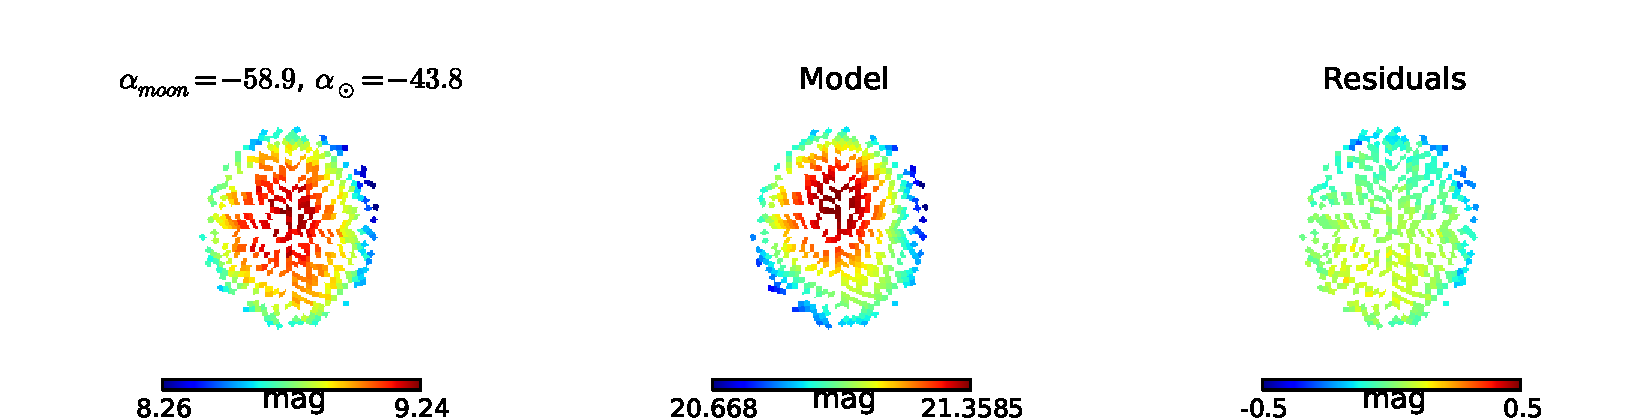
\includegraphics[height=5cm]{plots/exampleSkys_0.pdf} \\
  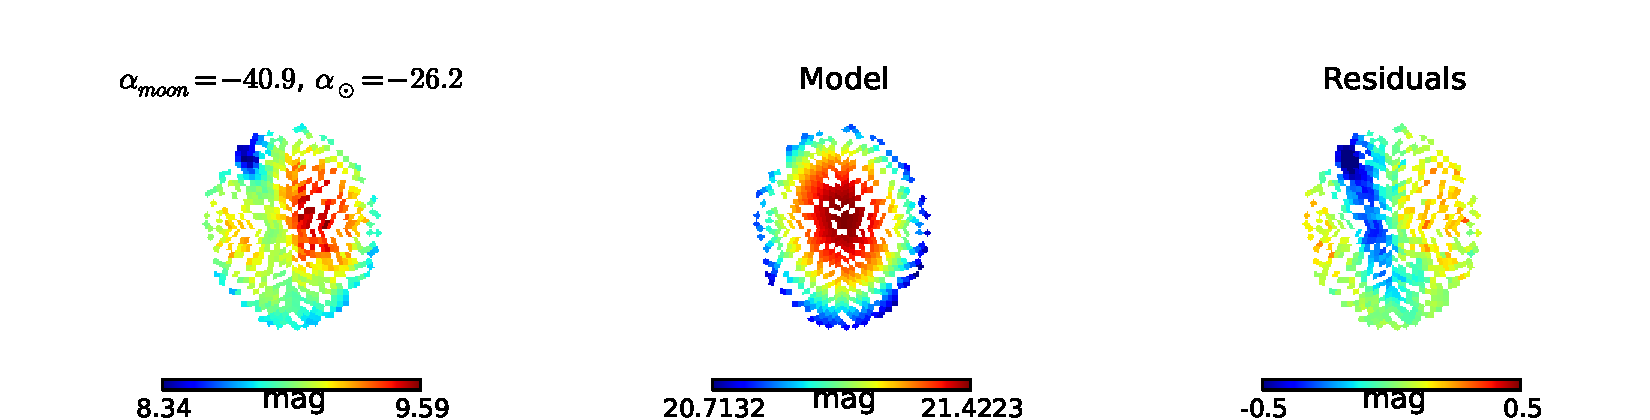
\includegraphics[height=5cm]{plots/exampleSkys_1.pdf} \\
  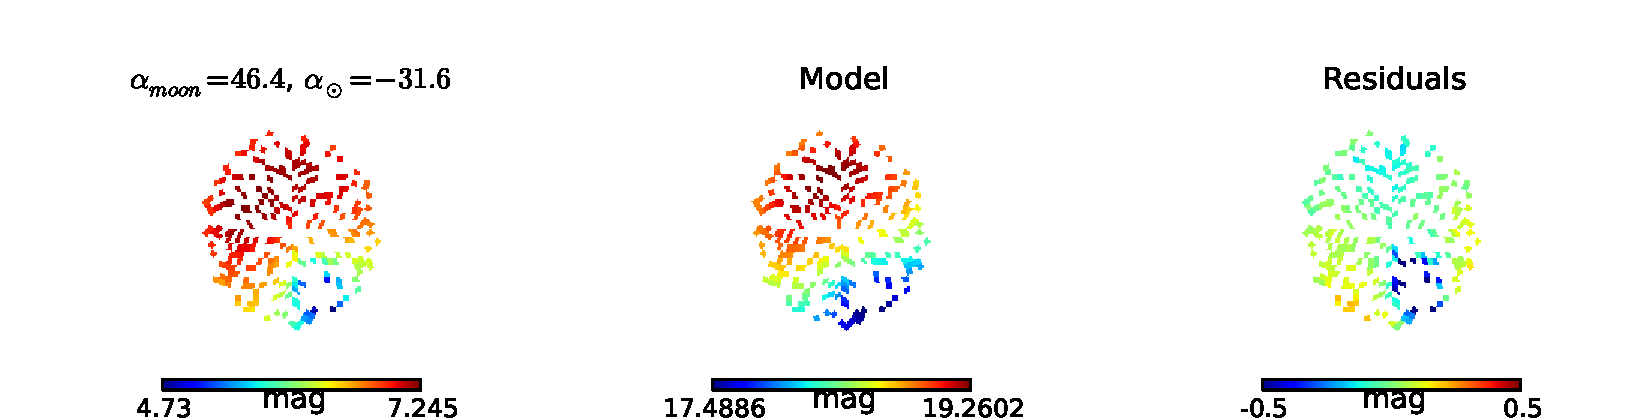
\includegraphics[height=5cm]{plots/exampleSkys_2.pdf} \\
  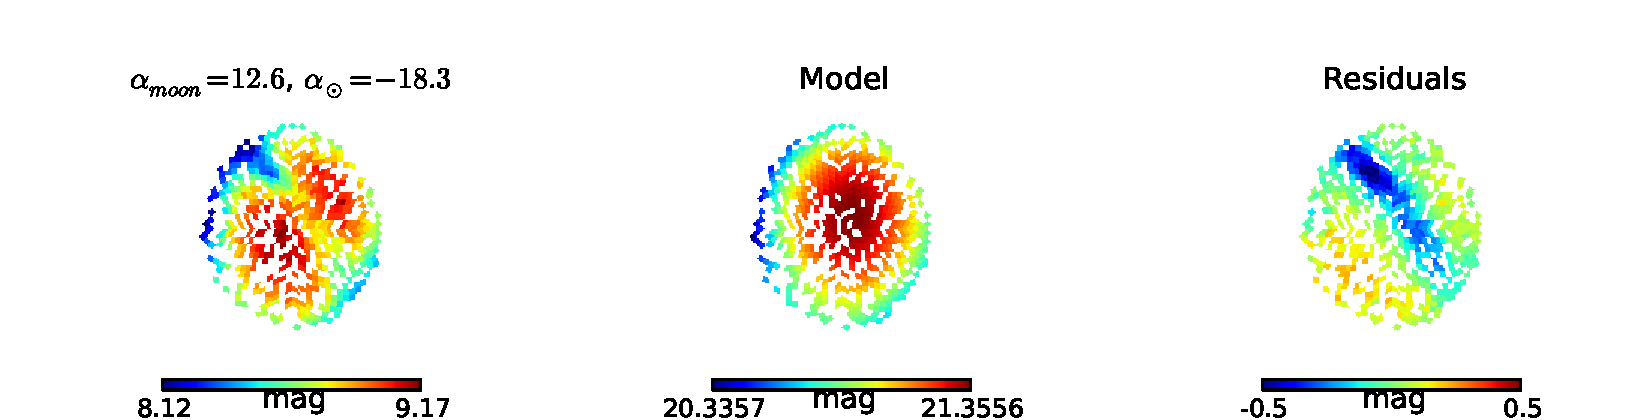
\includegraphics[height=5cm]{plots/exampleSkys_3.pdf}
  \end{center}
  \caption{Some examples of Canon all-sky observations and model values for airmasses less than 2.1. The sky observations have been binned into altitude-azimuth Healpixels (zenith at the center of the projections). These are all for the Canon R-filter. The top row shows a clear dark-time frame, the second row is a dark time frame where there were clouds. The third row shows a high moon, and the final row is during twilight with some light clouds. \label{fig:skyExamples}}
\end{figure*}


For the observations from the all-sky camera, we select those that have at least 200 stars detected to select those without extreme cloud extinction. To speed things up, we use every 10th frame from the sky camera, resulting in around 3400 unique observations.  We then bin the sky brightness observations onto a HEALpixel grid of nside=16 and compute the model sky brightness at each HEALpixel and zeropoint each frame (to correct for any average cloud cover or instrument zeropoint drift) and record the model and observation zenith sky brightness. Figure~\ref{fig:zenithModel} shows the median and standard deviation of the model and observation zenith residuals.  In general, the model does an excellent job matching the observed zenith sky brightness, and only fails when the moon is very high in the sky.  

\begin{figure*}[ht]
  \begin{center}
  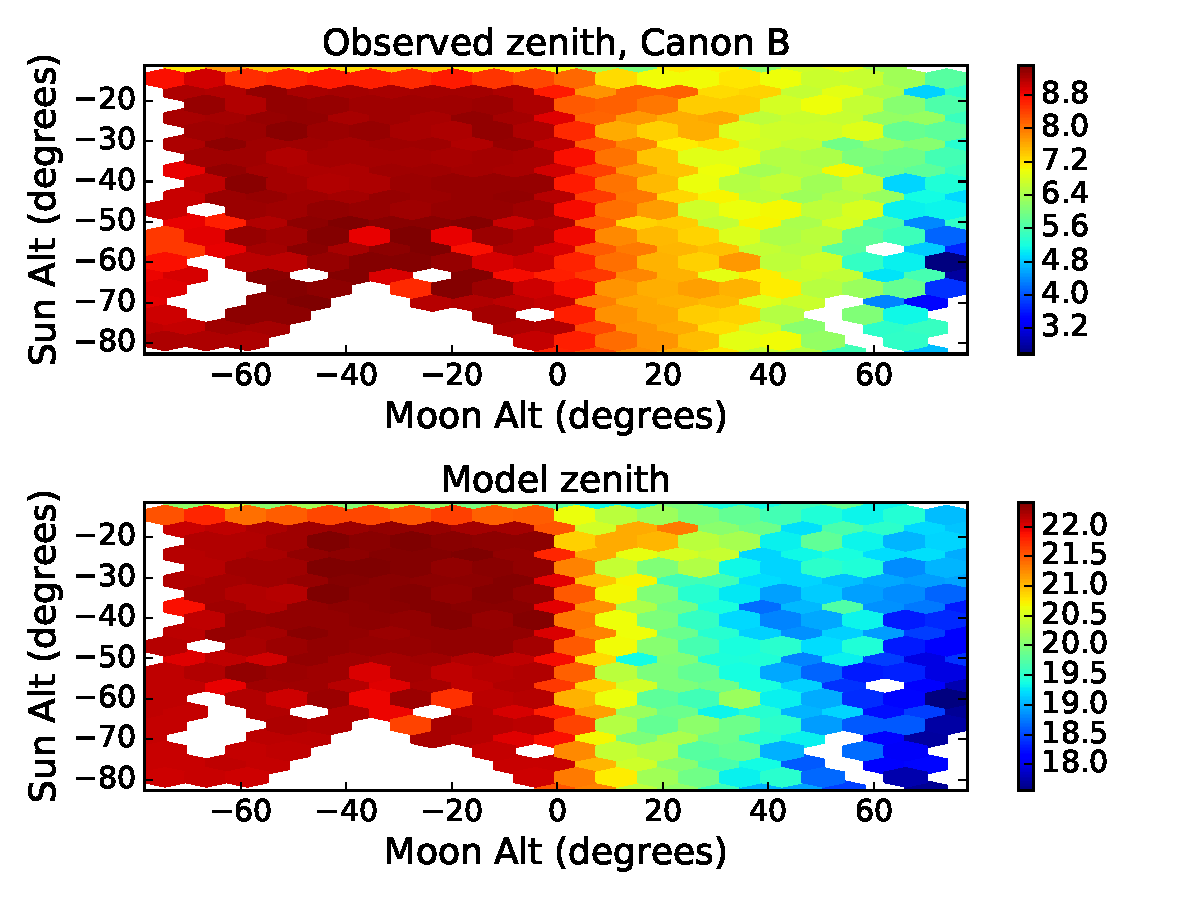
\includegraphics[height=5cm]{plots/simple_zenith_comp_B.pdf} 
  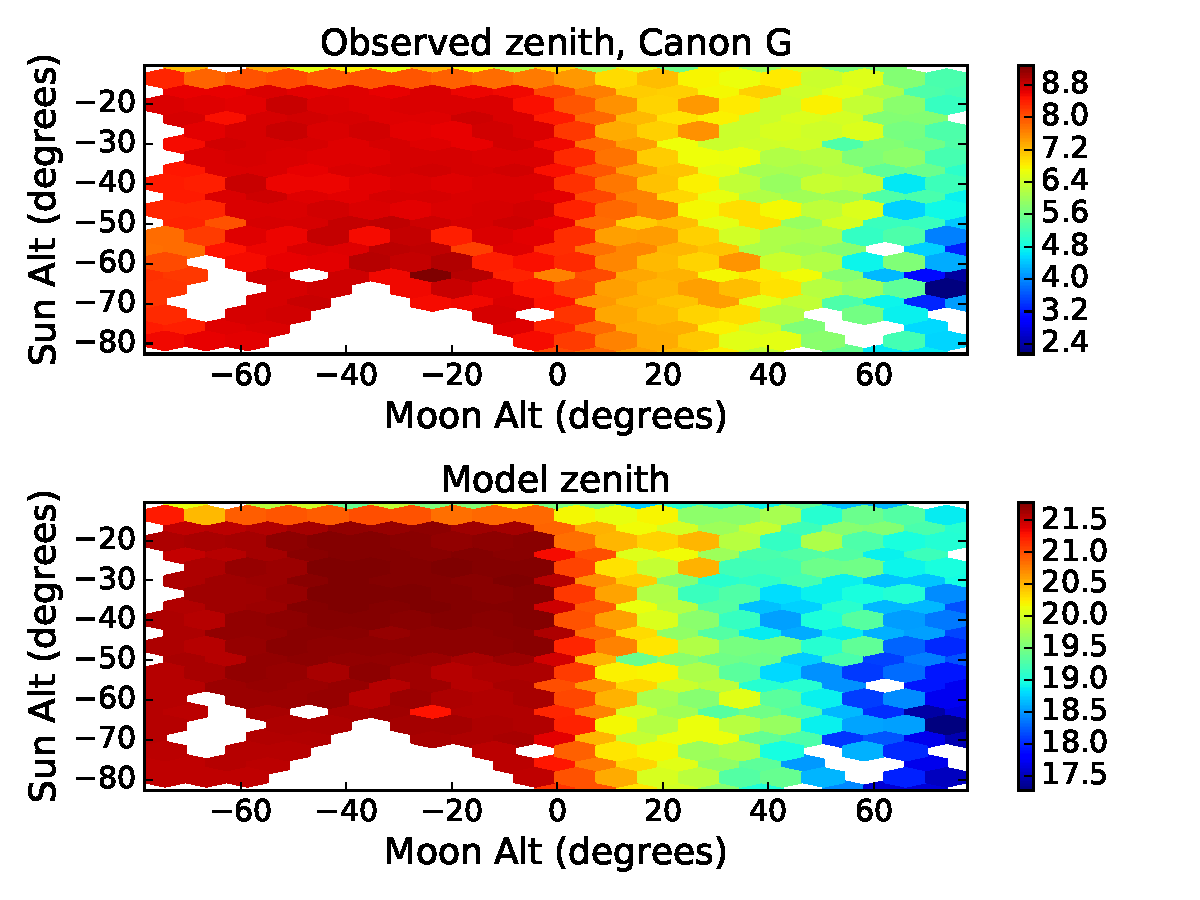
\includegraphics[height=5cm]{plots/simple_zenith_comp_G.pdf} 
  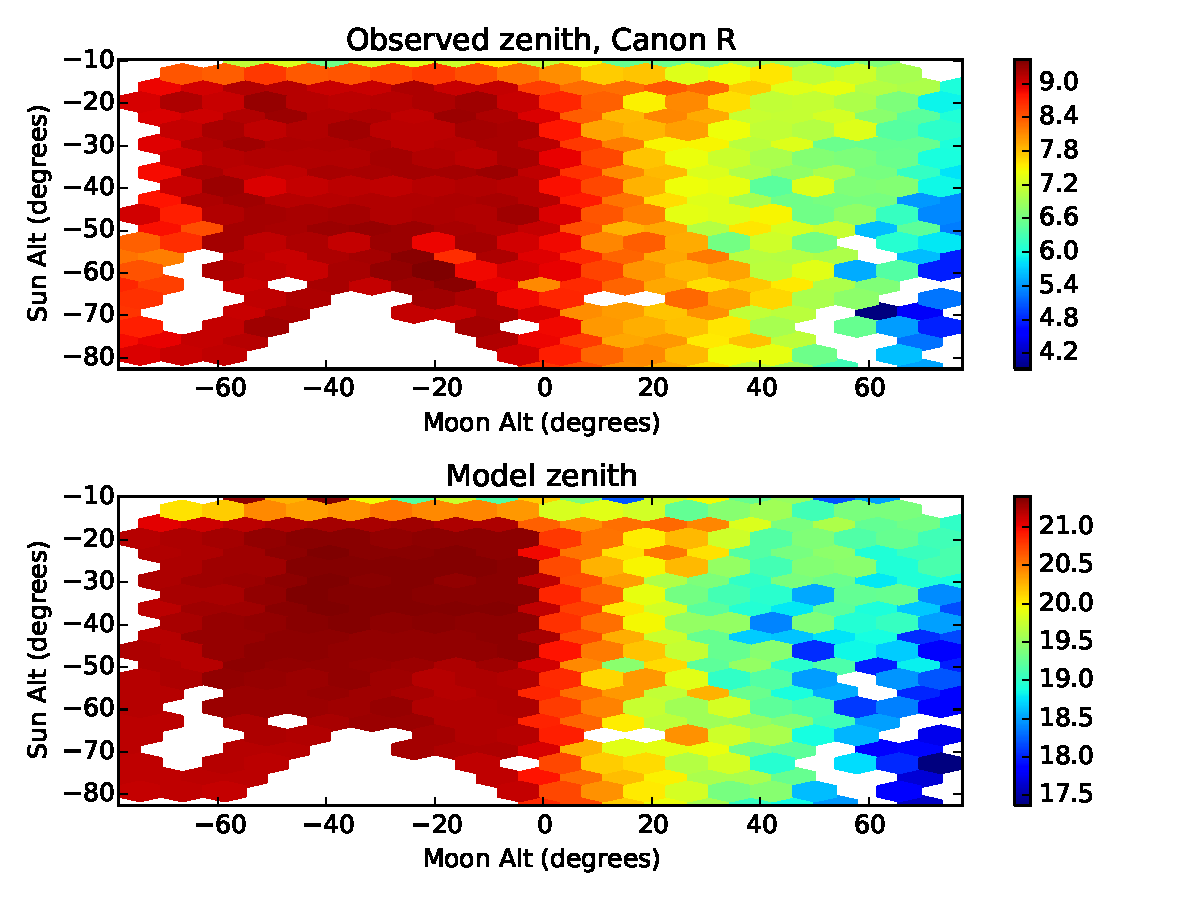
\includegraphics[height=5cm]{plots/simple_zenith_comp_R.pdf}
  \end{center}
  \caption{Comparing the Canon all-sky camera zenith observations (top rows) to the model (bottom rows). We have averaged over moon phases.  \label{fig:compareZenithCanon}}
\end{figure*}

% from validate.py
\begin{figure*}[ht]
  \begin{center}
  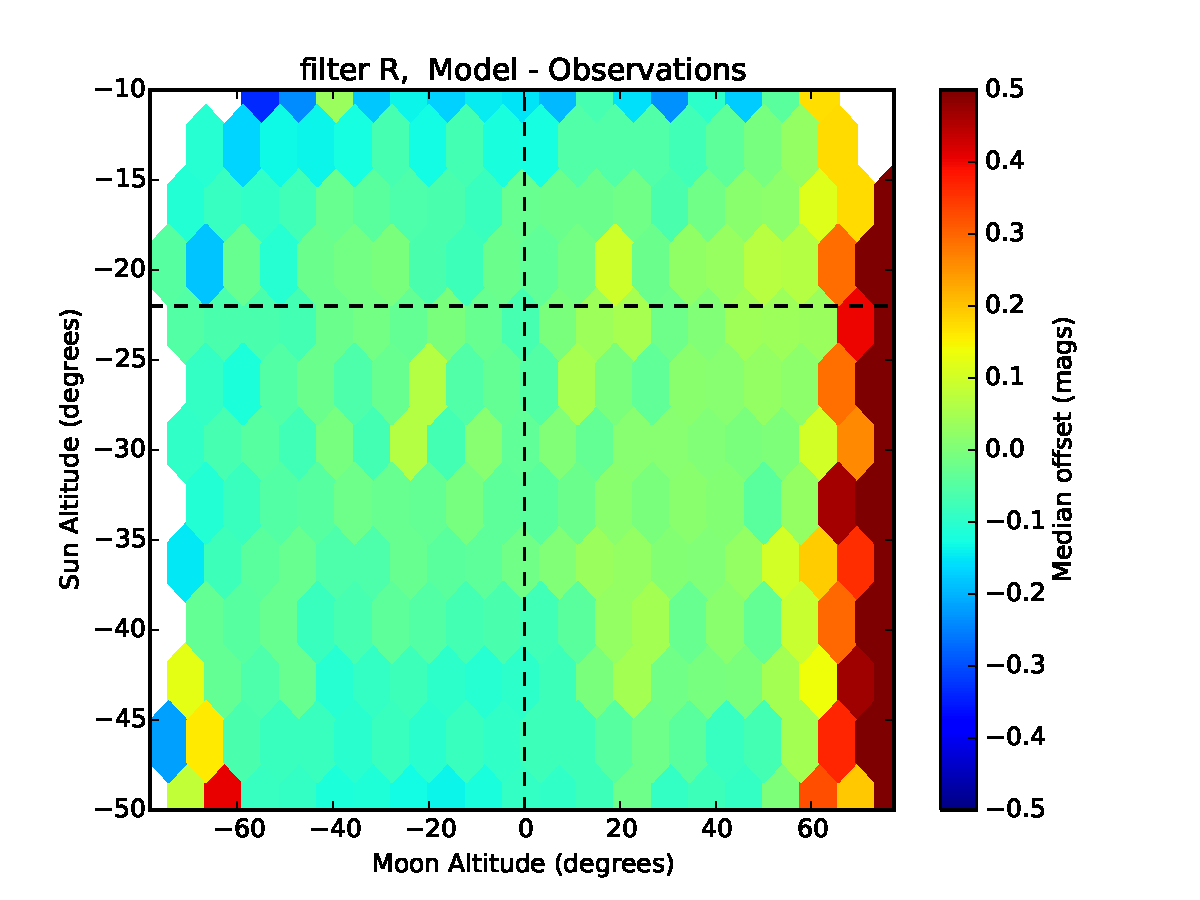
\includegraphics[height=5cm]{plots/zenithMedian_R_.pdf}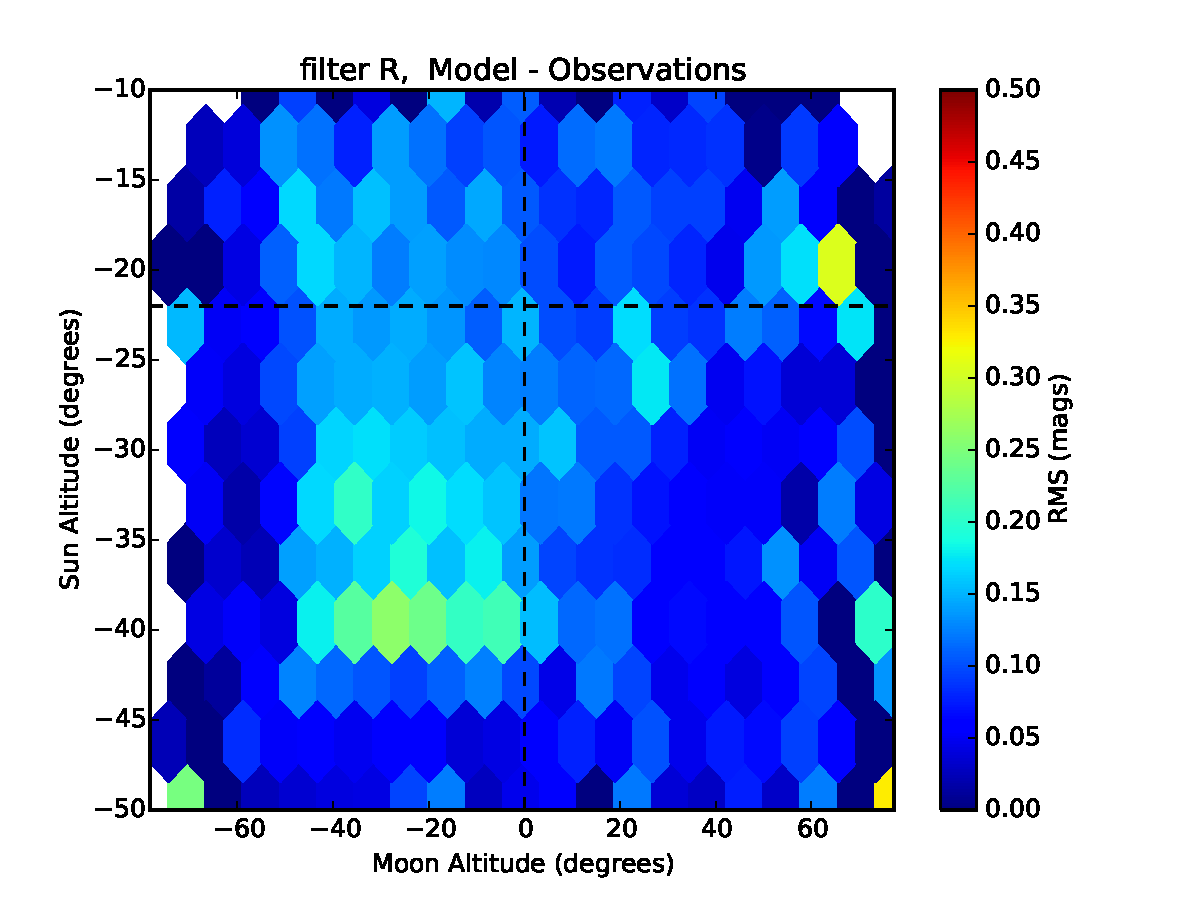
\includegraphics[height=5cm]{plots/zenithRMS_R_.pdf}
  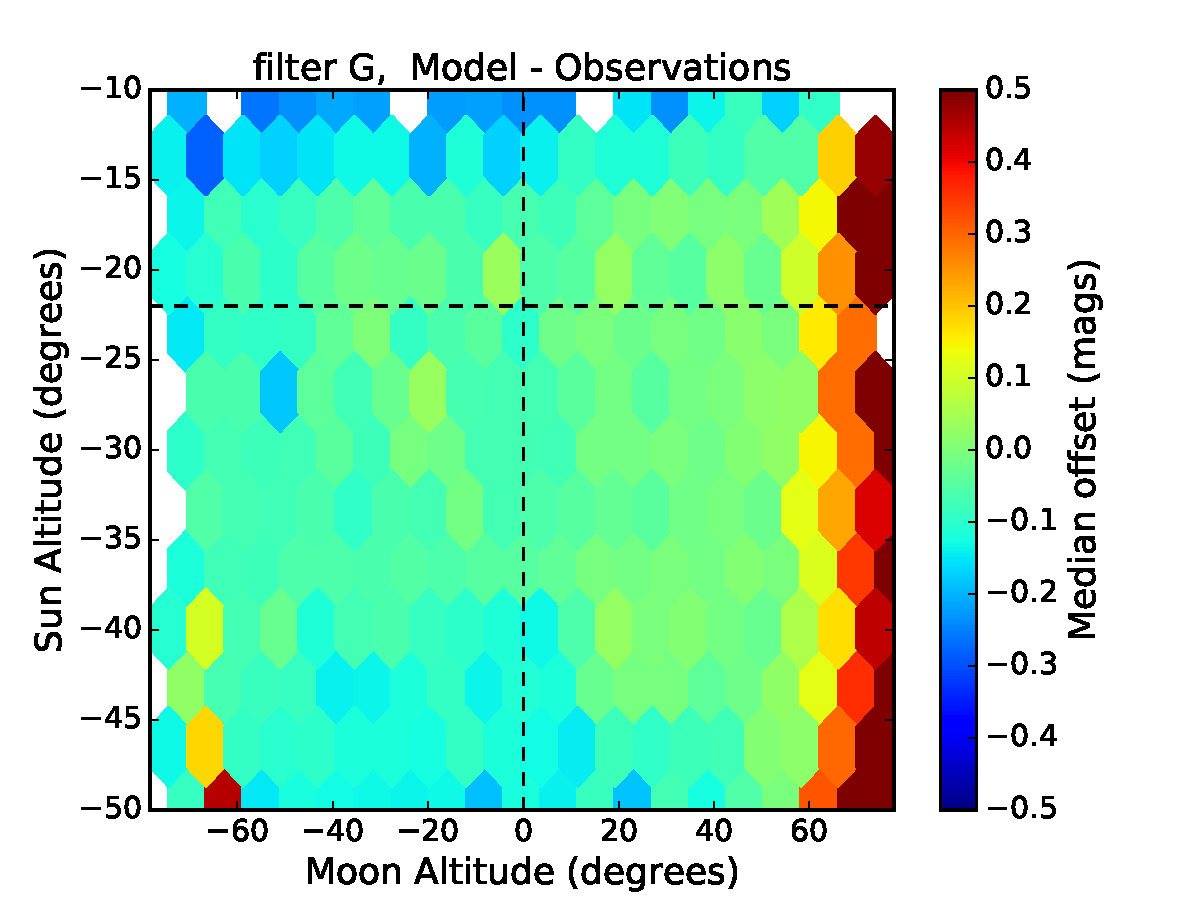
\includegraphics[height=5cm]{plots/zenithMedian_G_.pdf}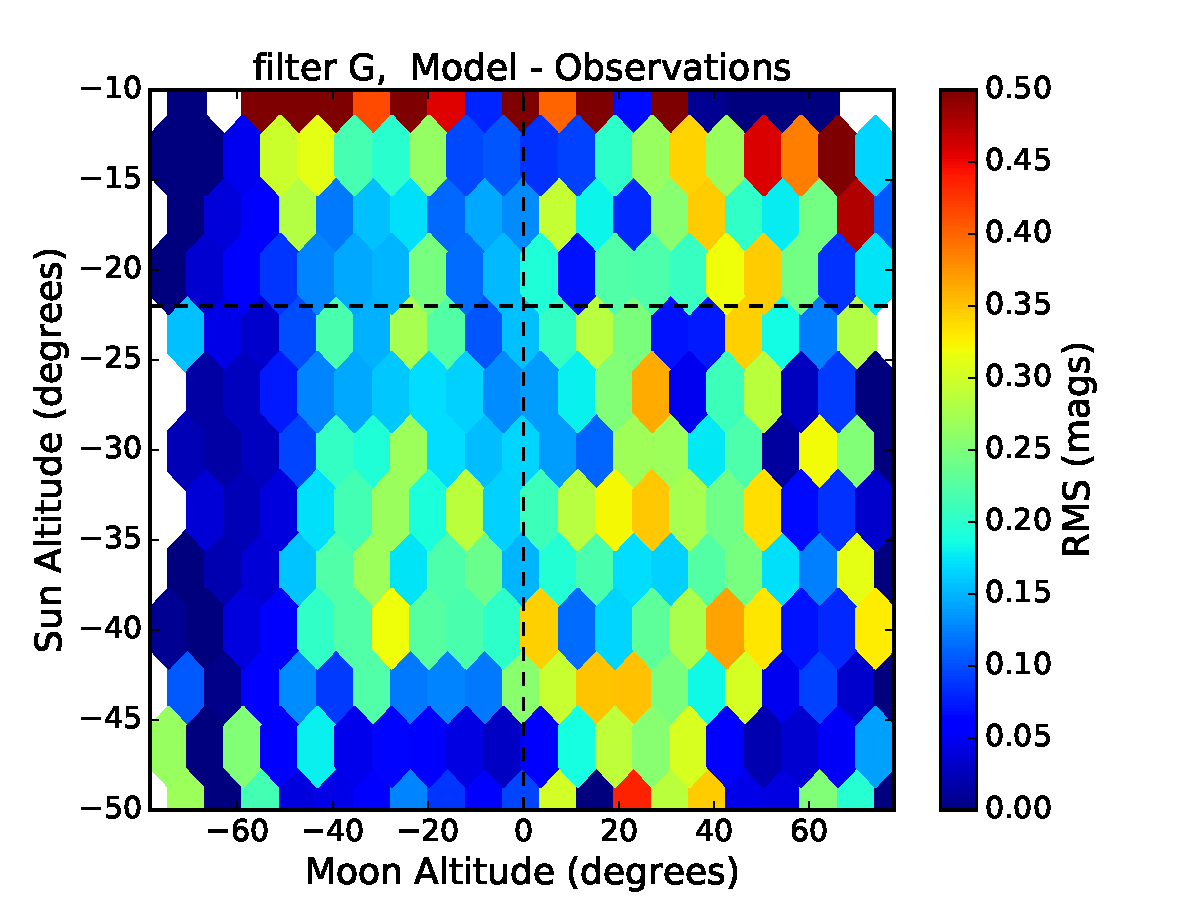
\includegraphics[height=5cm]{plots/zenithRMS_G_.pdf}
  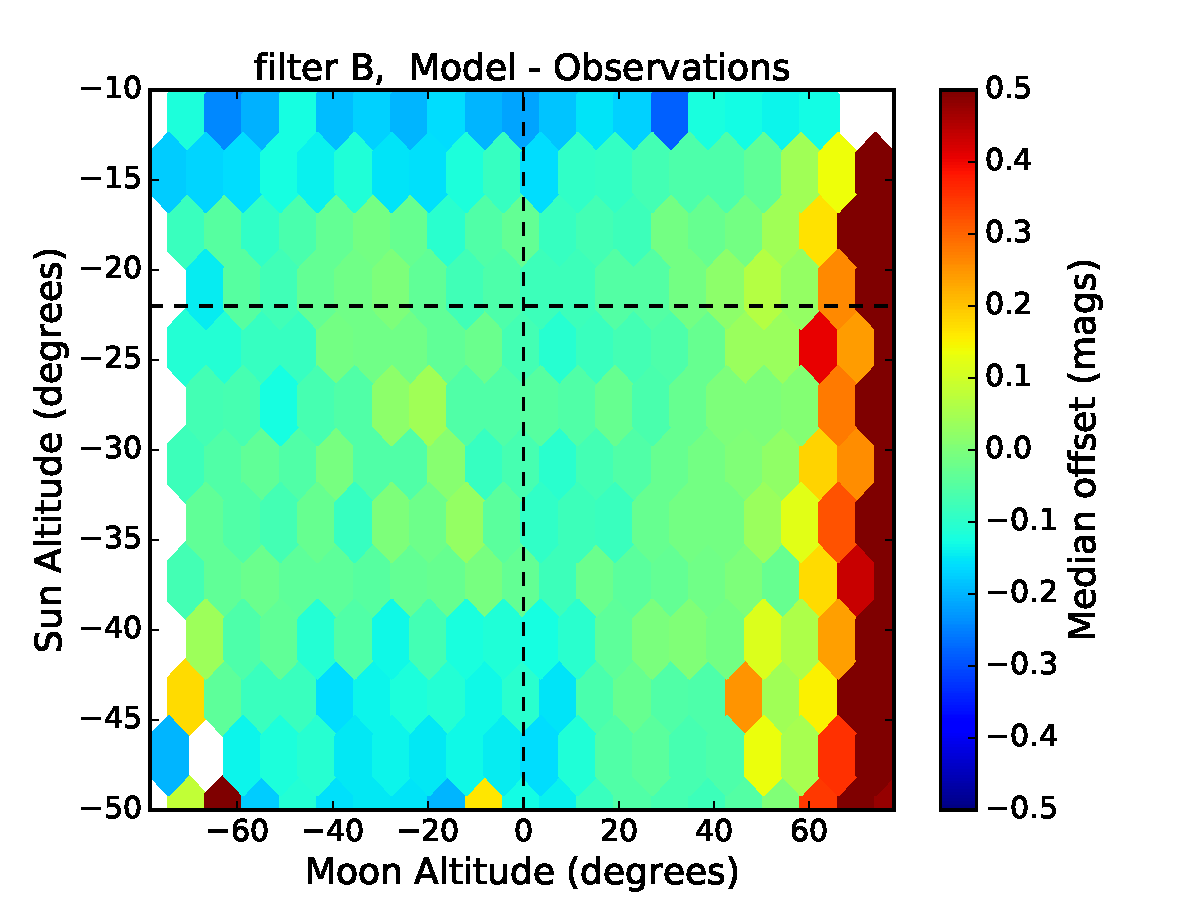
\includegraphics[height=5cm]{plots/zenithMedian_B_.pdf}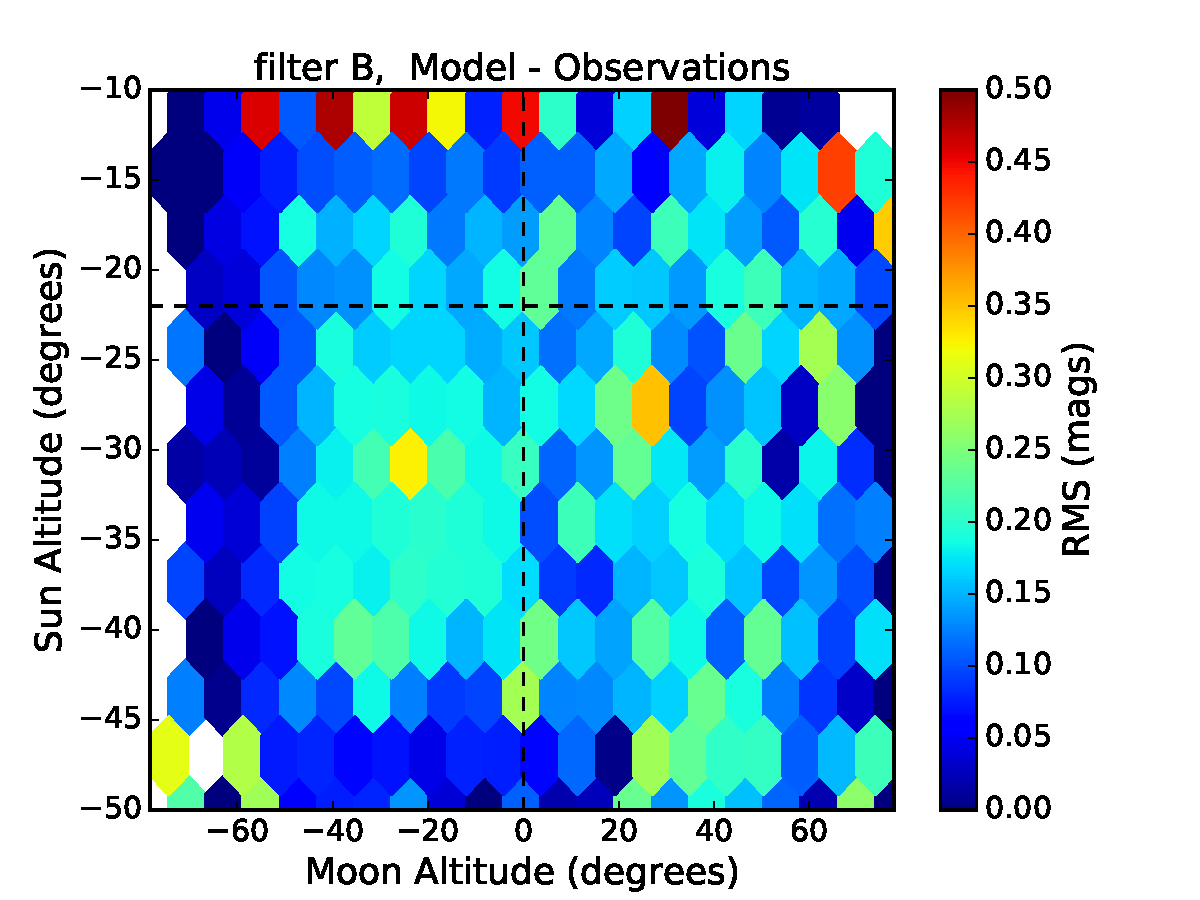
\includegraphics[height=5cm]{plots/zenithRMS_B_.pdf}
  \end{center}
  \caption{ The difference between the model predicted zenith sky brightness and the observed values from the Canon all-sky camera.  The model does tend to fail very near the moon, thus the large residuals when the moon reaches high is expected.  \label{fig:zenithModel}}
\end{figure*}


Our results can be compared to the ESO-Paranal twilight sky observations presented in Ref.~\citenum{Patat06}. We have scrapped the twilight zenith sky brightness data for observations taken of long-exposure standards with the FORS1 instrument.  The data and best fitting exponential-plus-constant models are shown in Figure~\ref{fig:Patat}.  The best-fit parameters are listed in Table~\ref{table:PatatFits}.  The Canon-B brightness seems to be fainter than Johnson's $B$.  The slopes of the twilight decay are very similar with the \cite{Patat06} data having $ -1.06  < a < -0.97 $ mag degree$^-1$ and our fits are in the range $ -1.02 < a < -0.97$ mag degree$^-1$.


In Table~\ref{table:darkSky}, we compare the median dark sky surface brightness computed from our model to the values adopted in Ref.~\citenum{Ivezic08}.  The only variation included in the model is from the changing impact of Zodiacal light.  Other than the $y$-band which disagrees by 0.5 magnitudes per square arcsecond, the model and \cite{Ivezic08} agree well. 

In Table~\ref{table:zenithRMSSky}, we list the (robust) RMS residuals between our model and the zenith sky brightness observed by the Canon all-sky camera. In general, the residuals between the model and observations have an RMS between 0.2 and 0.3 magnitude arcsecond$^{-2}$.  


% from checkDarkSky.py
\begin{table}
  \caption{Dark sky surface brightnesses }
  \label{table:darkSky}
  \begin{center}
  \begin{tabular}{c c  c}
  Filter & Model & Expected\cite{Ivezic08} \\
  & ($\mu$) &  ($\mu$)  \\
  \hline
  \hline
  $u$ &    22.81 $\pm$  0.04  &  22.90 \\
  $g$ &    22.27 $\pm$  0.11  &  22.30 \\
  $r$ &    21.25 $\pm$  0.08  &  21.20 \\
  $i$ &    20.38 $\pm$  0.04  &  20.50 \\
  $z$ &    19.40 $\pm$  0.02  &  19.60 \\
  $y$ &    18.10 $\pm$  0.01  &  18.60 
  \end{tabular}
  \end{center}
\end{table}


% from validate.py
\begin{table}
  
  \caption{ Robust RMS differences between the model and Canon sky observations in different conditions.}
  \label{table:zenithRMSSky}
  \begin{center}
  \begin{tabular}{c c c c}
  Filter & Dark Time & Moon Up & Twilight \\
  & (mags/sq arcsec)   & mags/sq arcsec) & (mags/sq arcsec) \\
  \hline
  \hline
  R & 0.22 & 0.24 & 0.29 \\
  G & 0.21 & 0.29 & 0.26 \\
  B & 0.22 & 0.38 & 0.26 
  \end{tabular}
  \end{center}
\end{table}


\begin{table}
  \caption{Parameter fits to data from Ref.~\citenum{Patat06}}
  \label{table:PatatFits}
  \begin{center}
  \begin{tabular}{c c c}
  Filter & $r_{12/z}$ & $a$  \\
  & & (1/radians) \\
  \hline
  \hline
  U & 13.40 & 22.37 \\
  B & 15.49 & 22.60 \\
  V & 4.78  & 22.31 \\
  R & 3.35  & 24.35 \\
  I & 2.29  & 24.08
\end{tabular}
\end{center}
\end{table}


\begin{figure}[ht]
  \begin{center}
  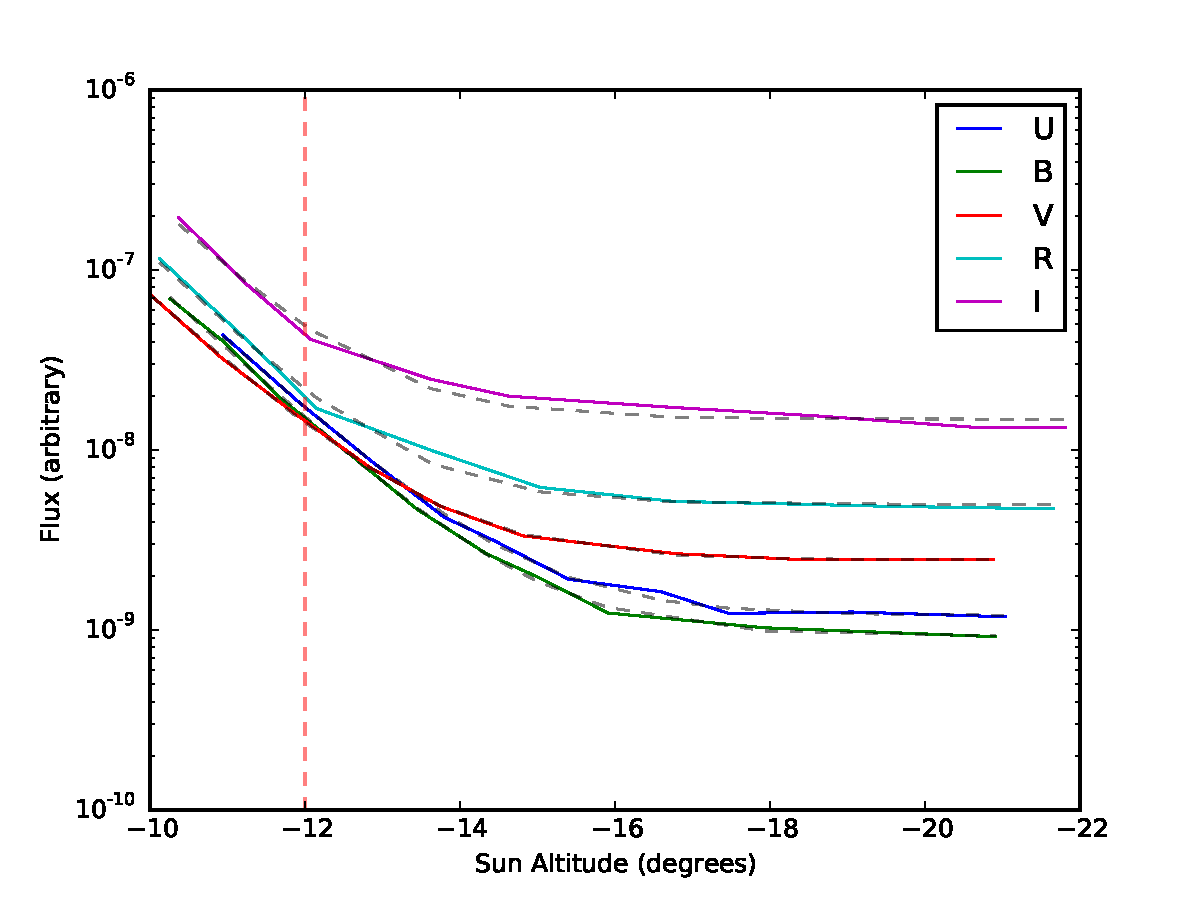
\includegraphics[height=5cm]{plots/patatFits.pdf}
  \end{center}
  \caption{Zenith sky surface brightness data scraped from Ref.~\citenum{Patat06} and fit with our simple exponential decay plus constant model. Dashed black lines show the best-fit curves.  The red dashed line shows the 12-degree twilight line.  \label{fig:Patat} }
\end{figure}

\clearpage

In Figures~\ref{fig:timeOfNight} and~\ref{fig:timeOfYear} we look at the observed and predicted zenith sky brightness during dark time as a function of the time of night and the time of year.  We also plot the adopted instrumental magnitude zeropoint, as the zeropoint could absorb changes in the sky brightness that were not correctly modeled.  There are no obvious trends in the plots, suggesting that adding terms to model the seasonal and nightly variations in the sky would not significantly improve our accuracy.  The zenith residuals do show a $\sim-0.15$ magnitude offset, suggesting a small error in how well we fit the airmass dependence.  This is probably just the result of there being many more high airmass pixels than zenith pixels, so a small error at high airmass can bias the computed frame zeropoint. It is also possible the zenith brightness extends slightly below the Canon noise floor.

We can also compare our model to various published observations of the night sky brightness.  Ref.~\citenum{Galaz15} observing a high-airmass target with Magellen in dark time report average sky brightnesses of $r=20.2$ and $g=21.8$ mag arcsec$^{-2}$.  Running our sky model, we find  $r=20.8$ and $g=22.0$ mag arcsec$^{-2}$--very similar in the $g$ band, and the model is 0.6 mags fainter in $r$.  Not too surprising since we expect the model to break down at higher airmasses in general.

\begin{figure*}[ht]
  \begin{center}
  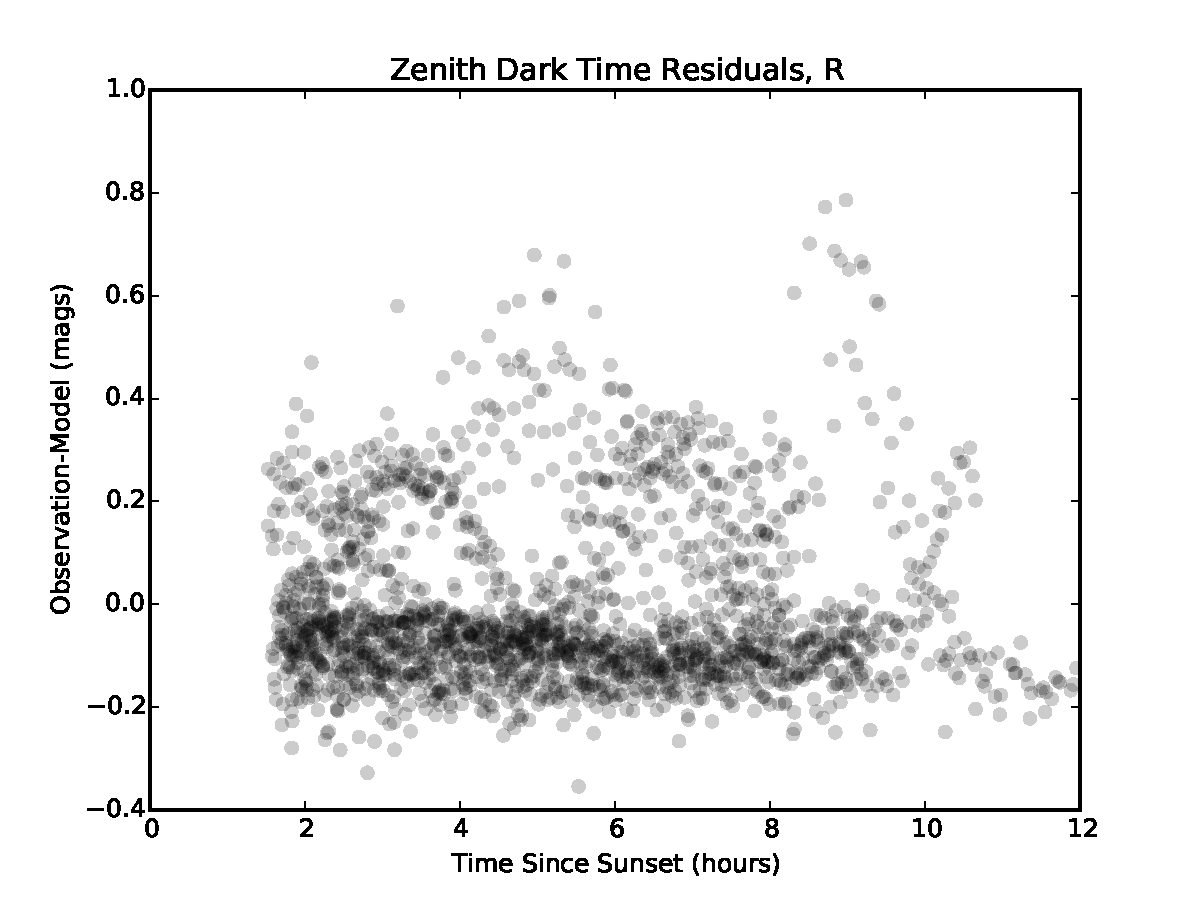
\includegraphics[height=4cm]{plots/residTON_R.pdf}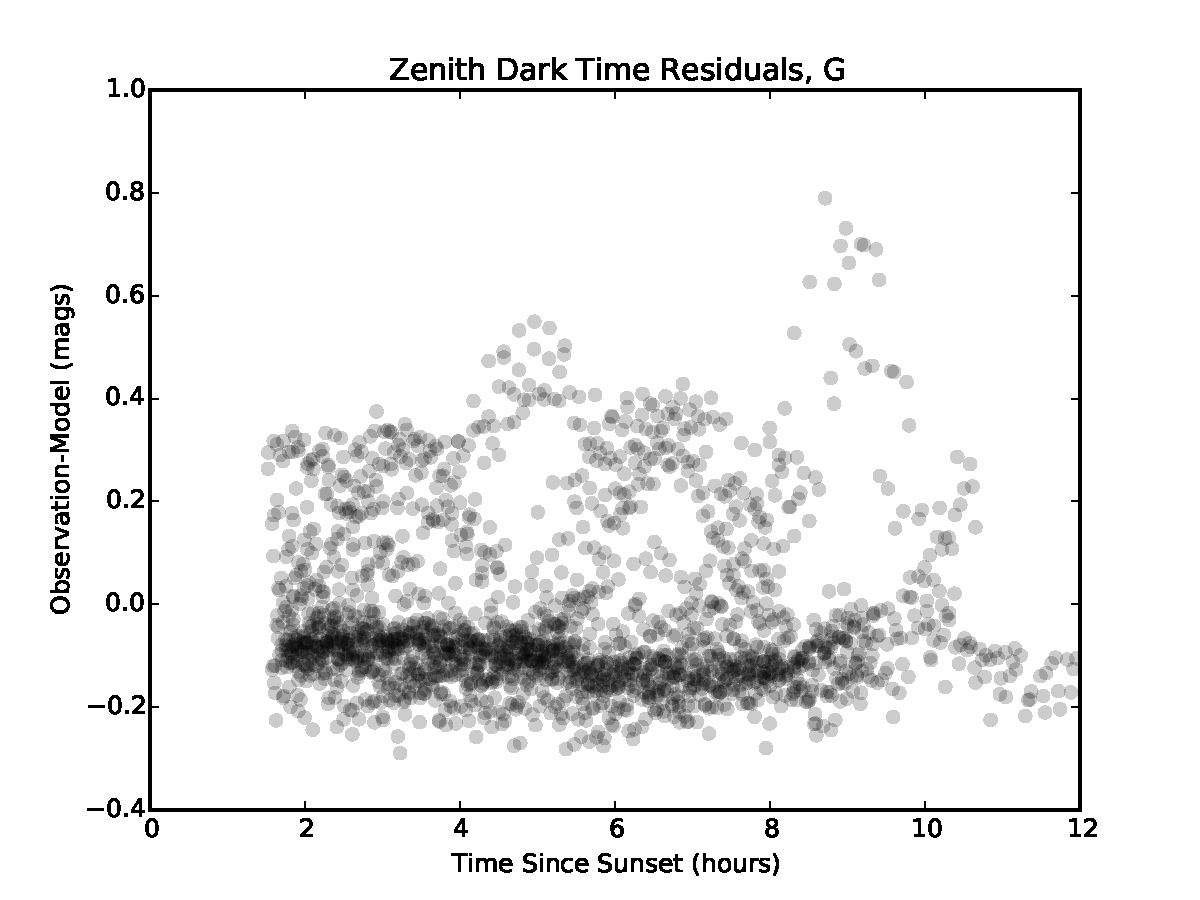
\includegraphics[height=4cm]{plots/residTON_G.pdf}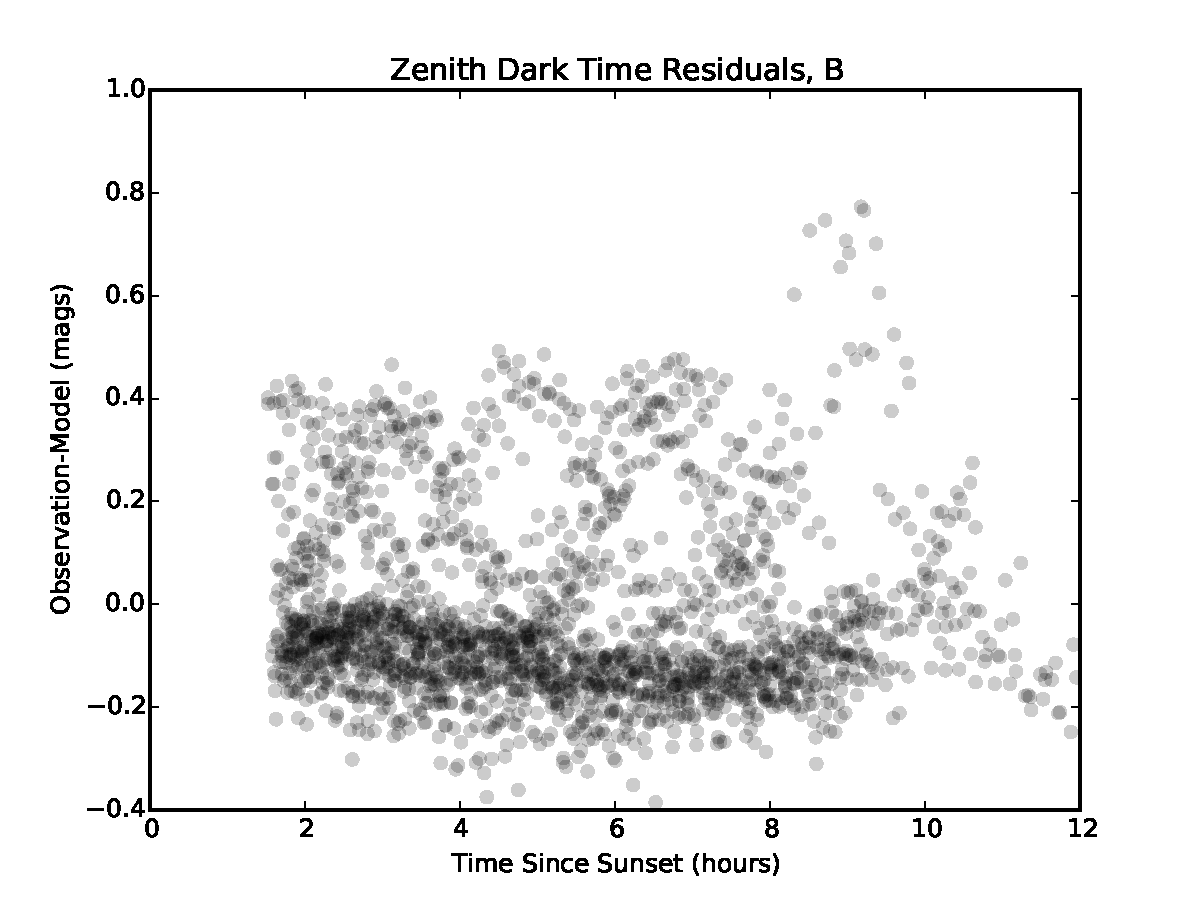
\includegraphics[height=4cm]{plots/residTON_B.pdf} \\
  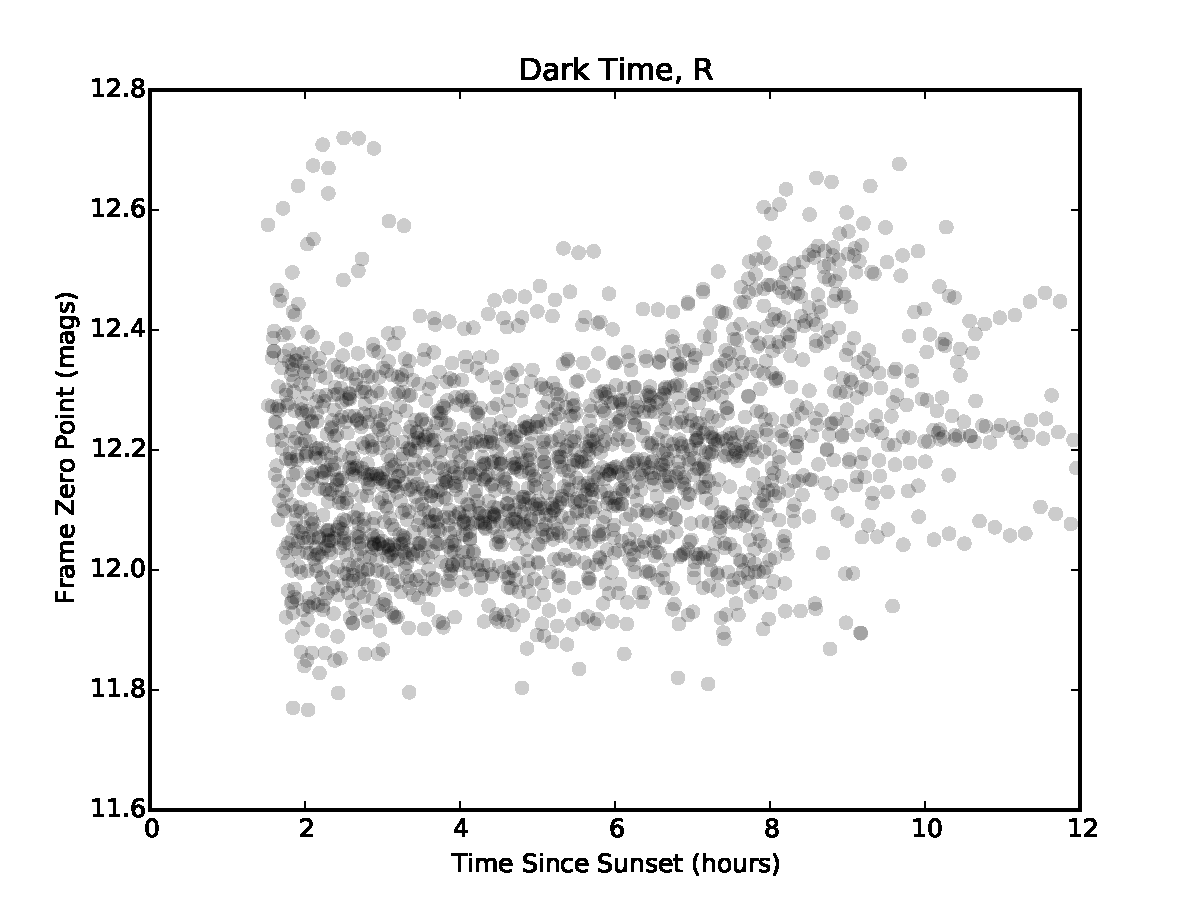
\includegraphics[height=4cm]{plots/zpTON_R.pdf}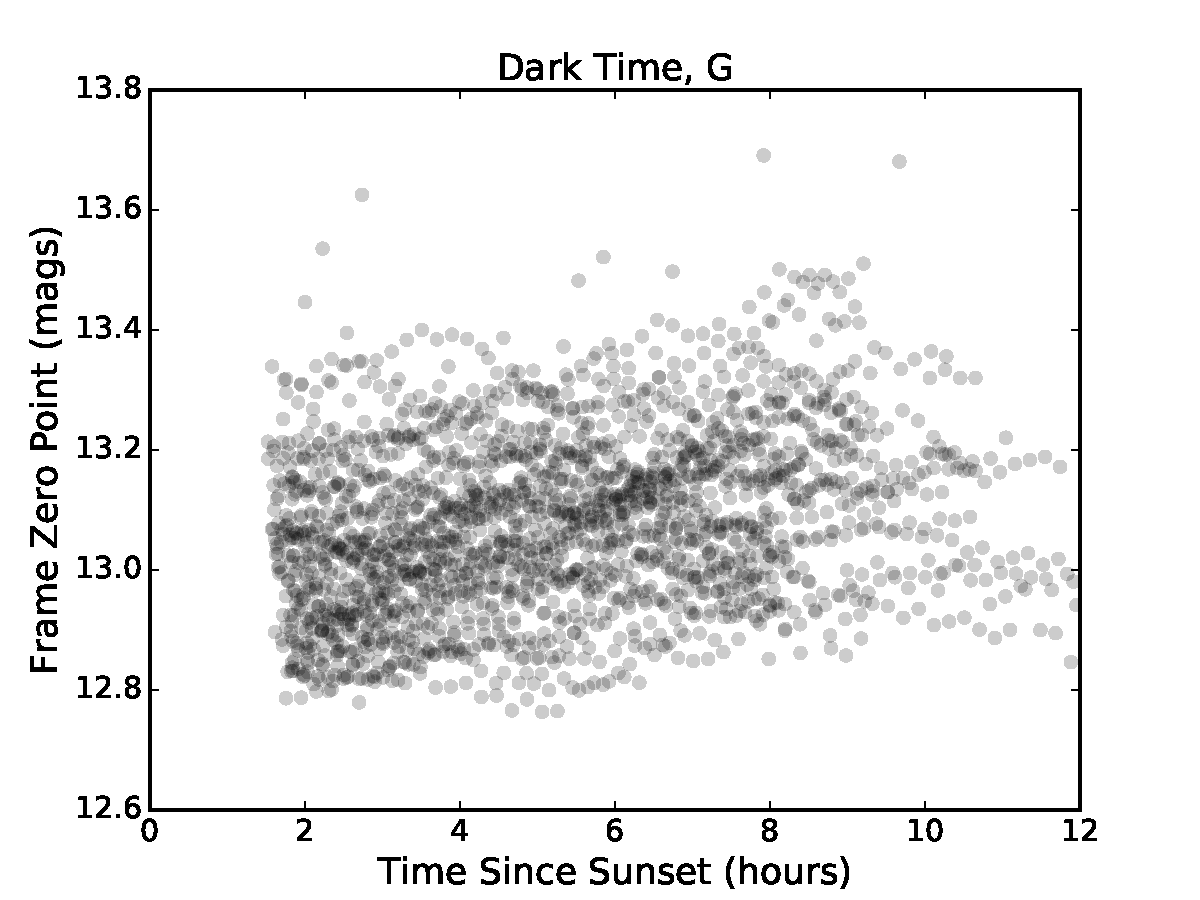
\includegraphics[height=4cm]{plots/zpTON_G.pdf}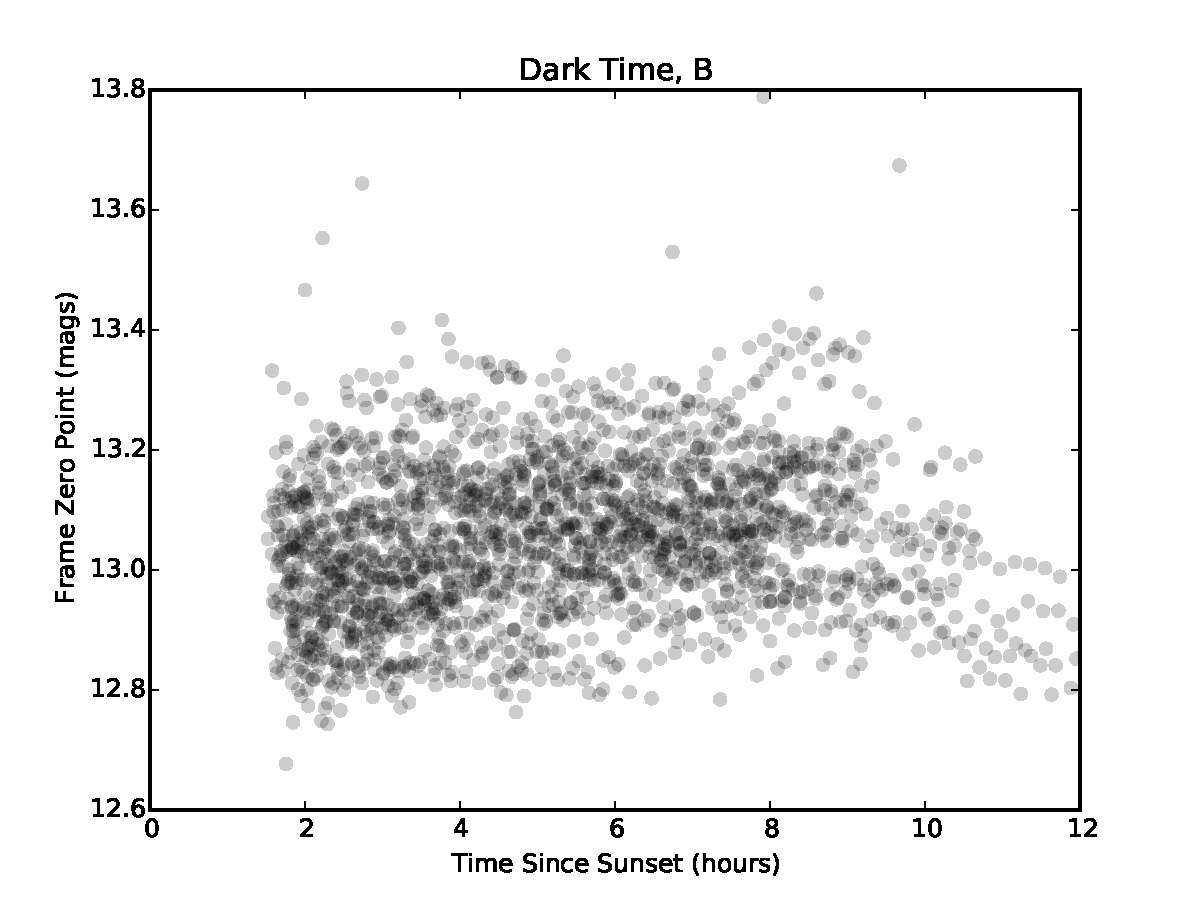
\includegraphics[height=4cm]{plots/zpTON_B.pdf}
  \end{center}
  \caption{The Canon camera zenith sky brightness residuals along with the adopted magnitude zeropoint for each frame. The outlier residuals at large values are most likely times when there were clouds at zenith.  \label{fig:timeOfNight}}
\end{figure*}

\begin{figure*}[ht]
\begin{center}
  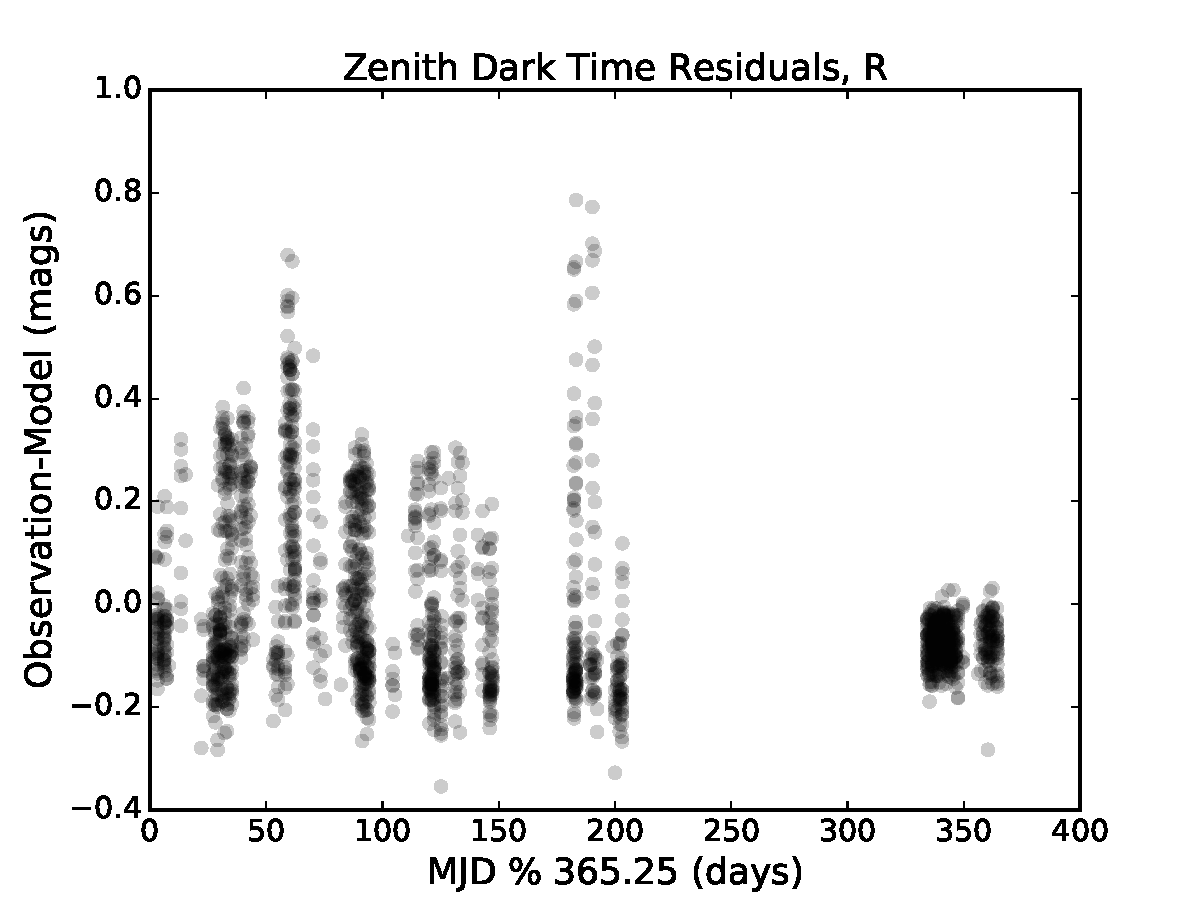
\includegraphics[height=4cm]{plots/residTOY_R.pdf}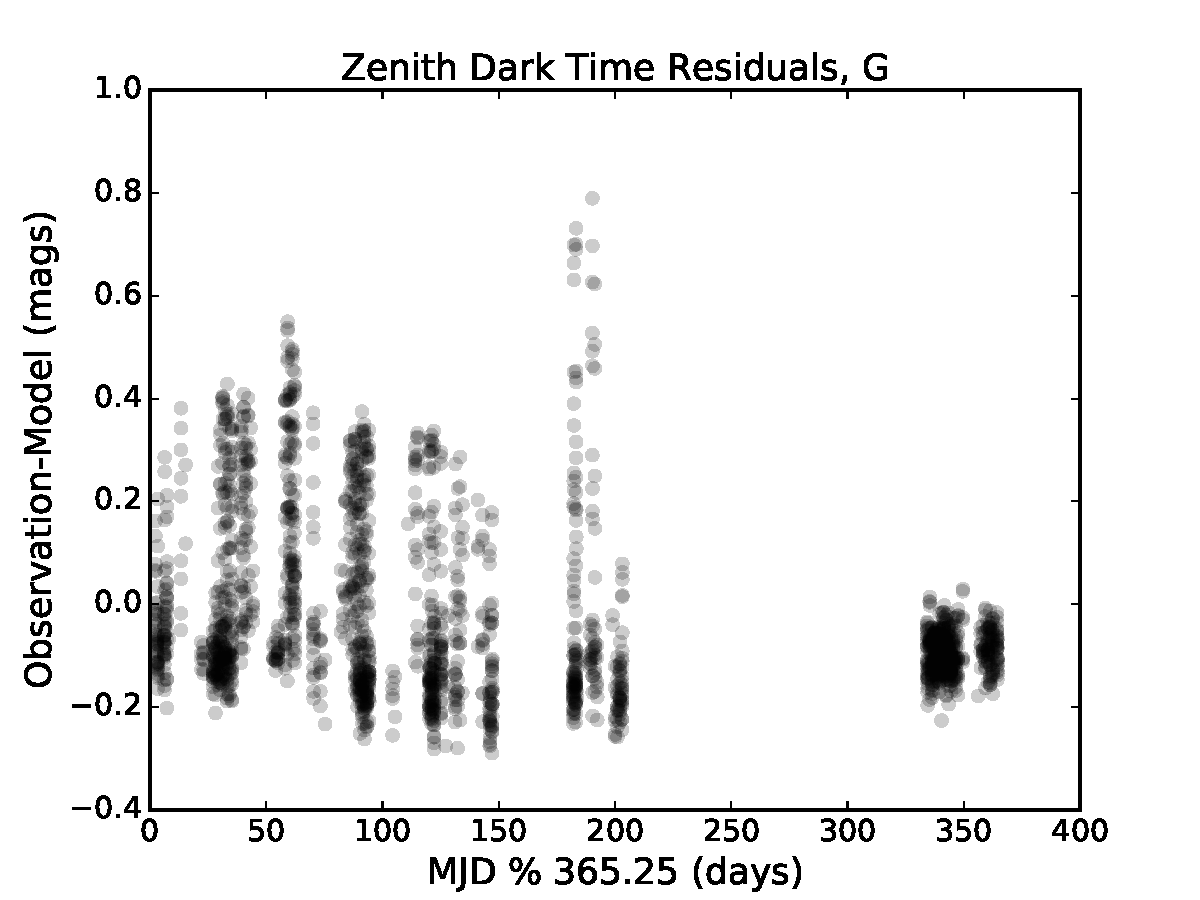
\includegraphics[height=4cm]{plots/residTOY_G.pdf}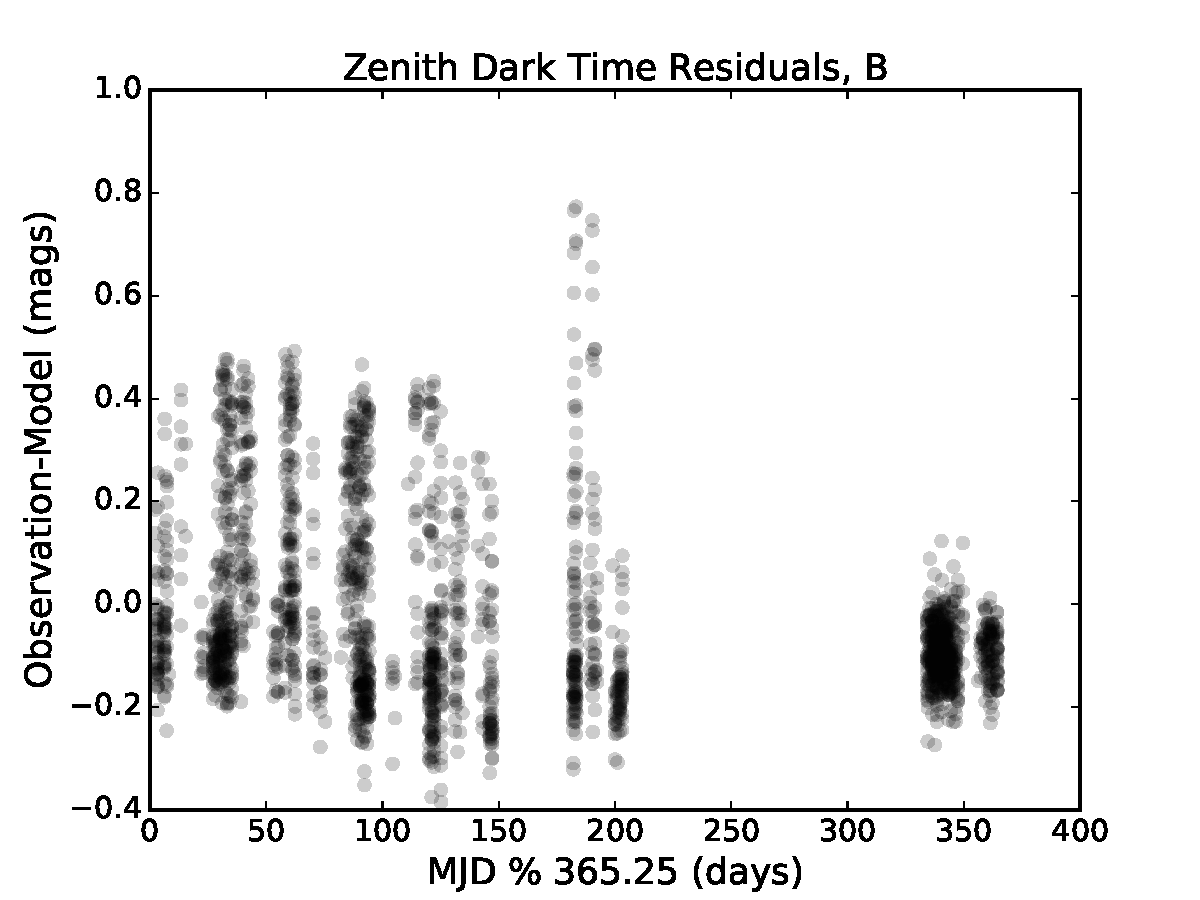
\includegraphics[height=4cm]{plots/residTOY_B.pdf} \\
  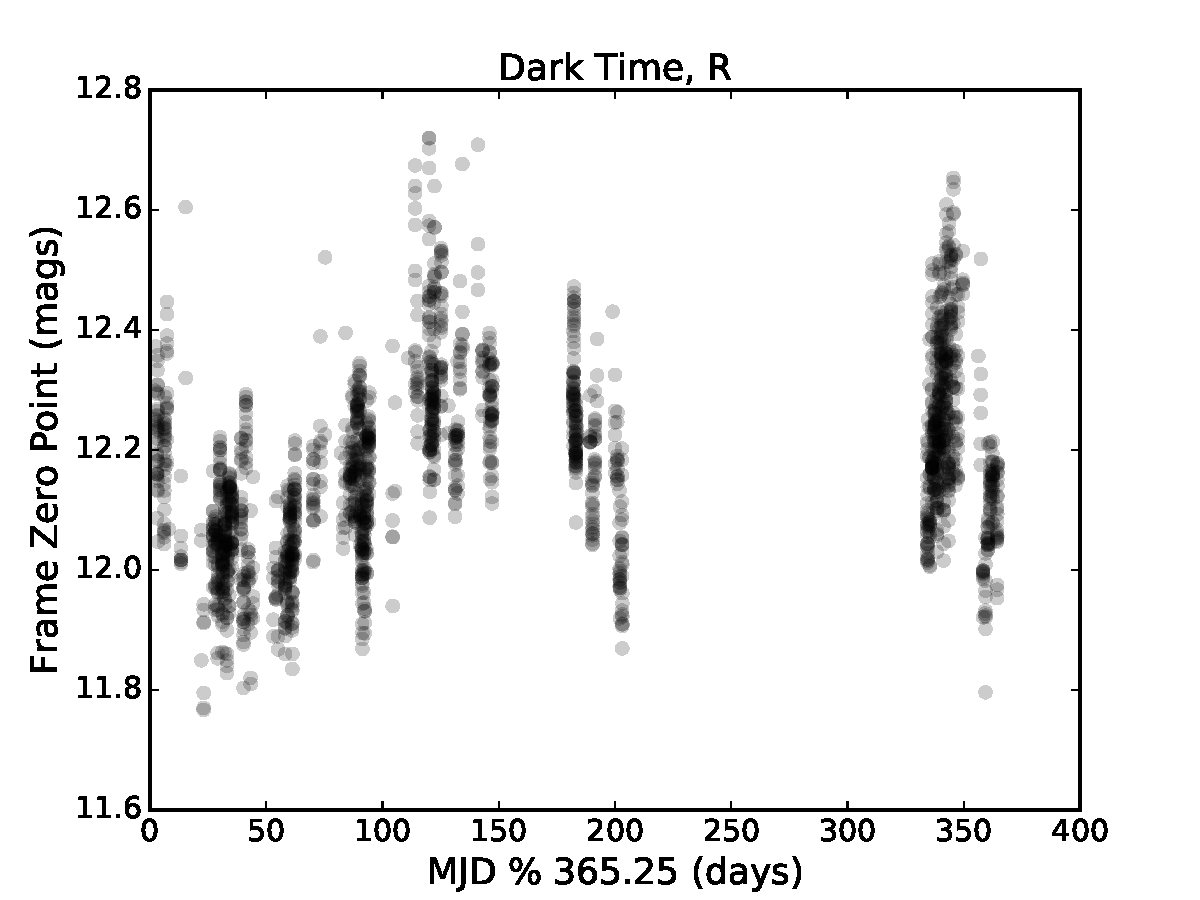
\includegraphics[height=4cm]{plots/zpTOY_R.pdf}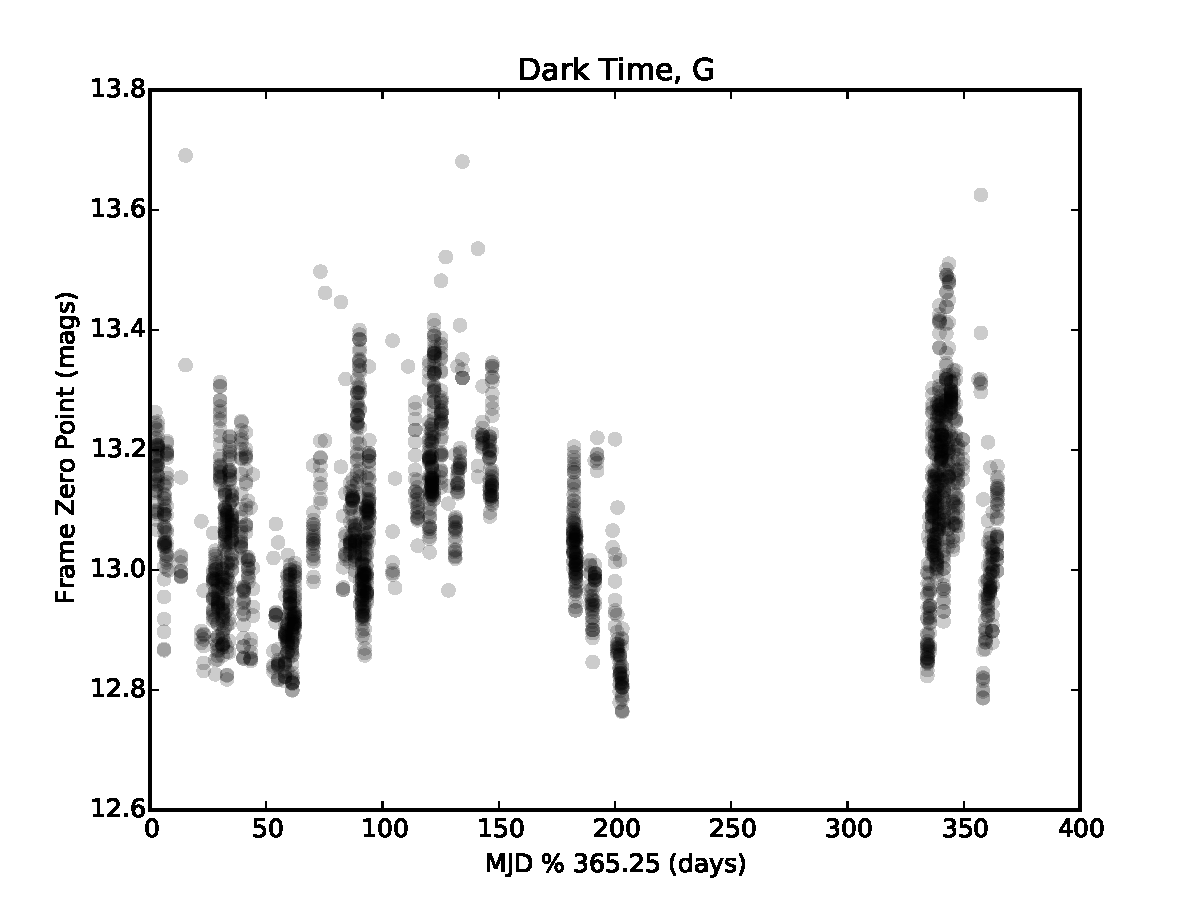
\includegraphics[height=4cm]{plots/zpTOY_G.pdf}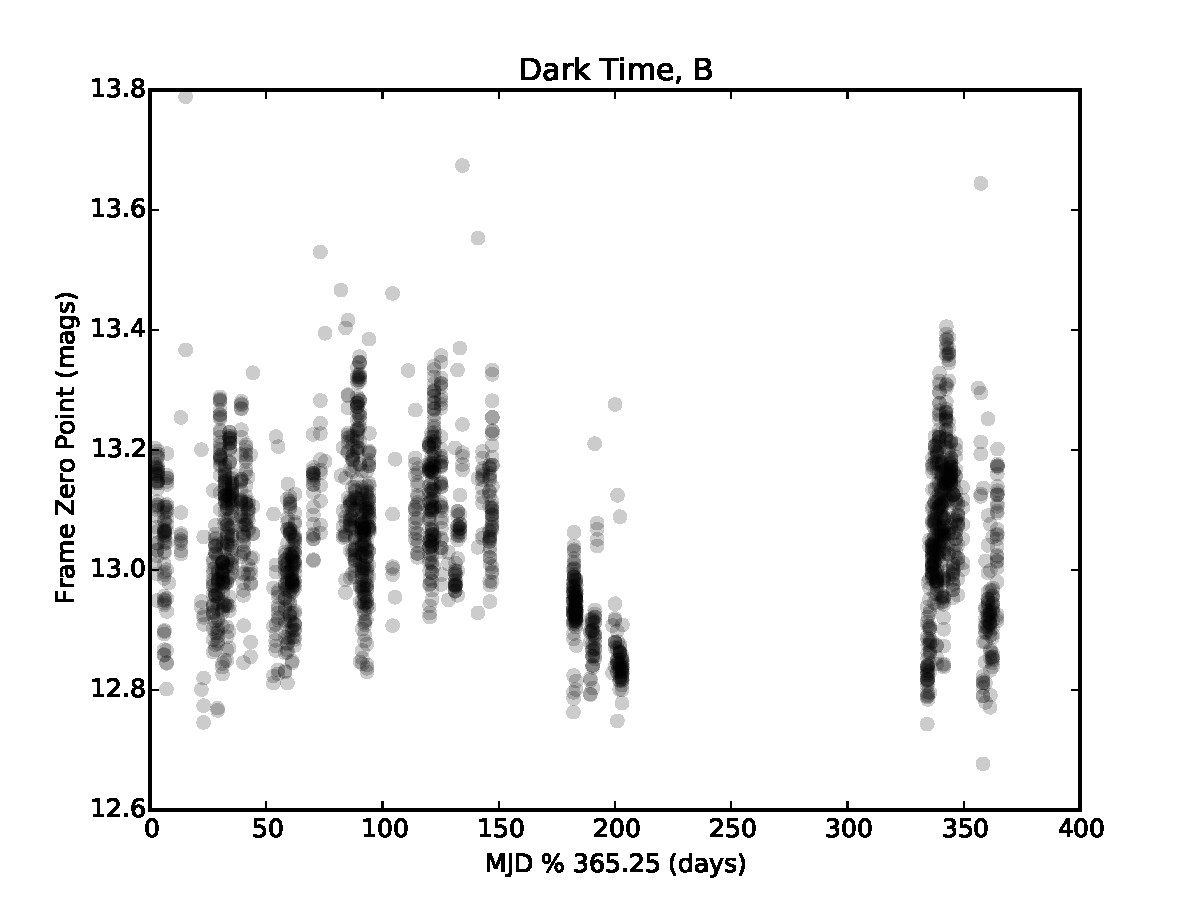
\includegraphics[height=4cm]{plots/zpTOY_B.pdf}
  \end{center}
  \caption{The Canon camera zenith sky brightness residuals along with the adopted magnitude zeropoint for each frame. \label{fig:timeOfYear}}
\end{figure*}



\begin{figure*}[ht]
\begin{center}
  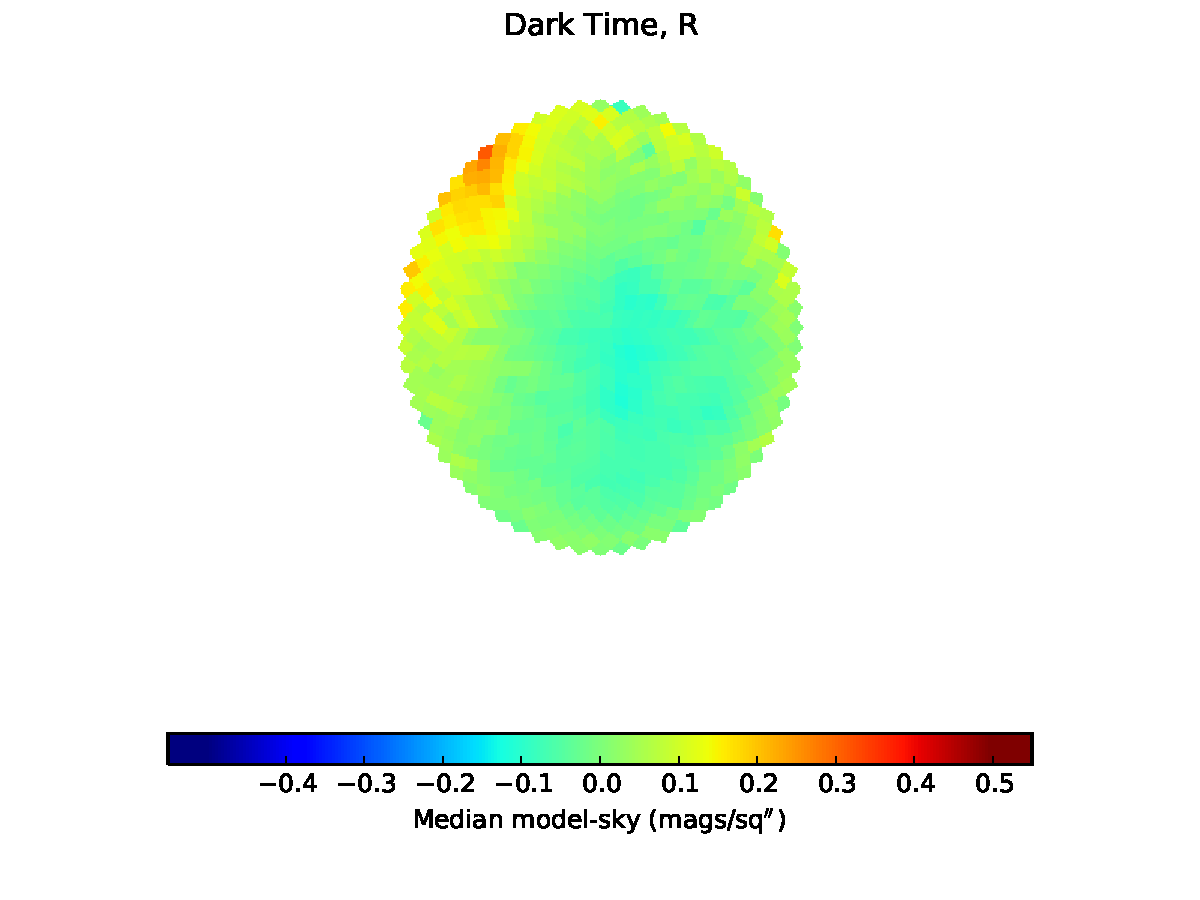
\includegraphics[height=5cm]{plots/medianResidMap_R.pdf}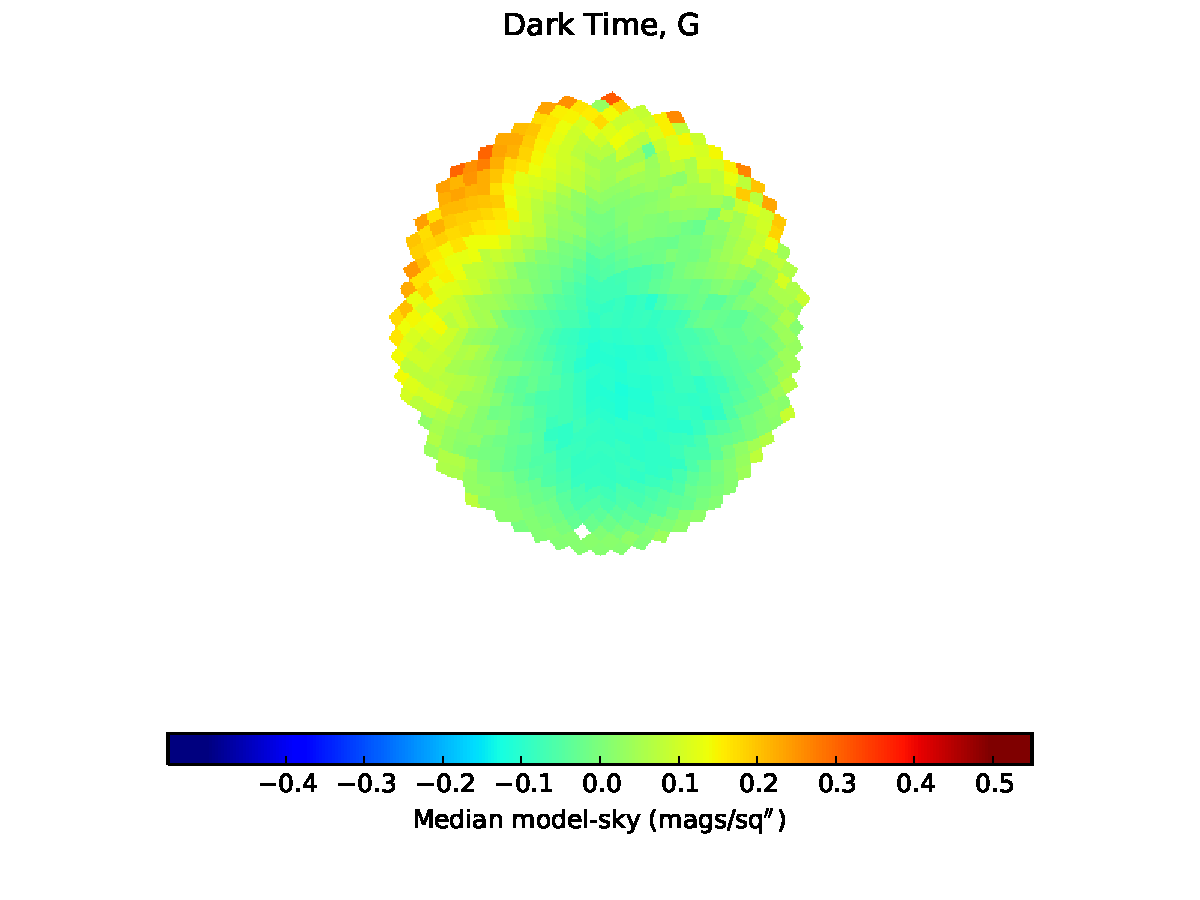
\includegraphics[height=5cm]{plots/medianResidMap_G.pdf}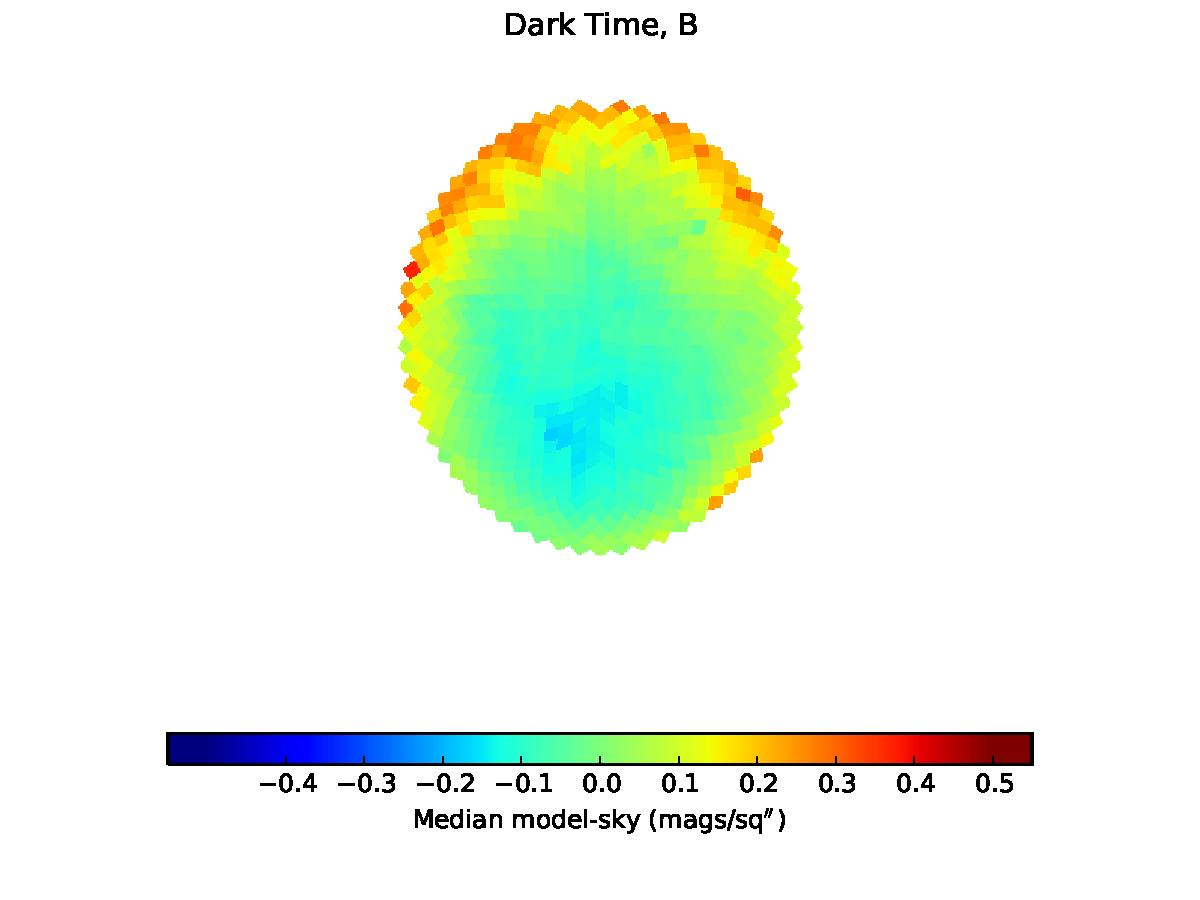
\includegraphics[height=5cm]{plots/medianResidMap_B.pdf} \\
  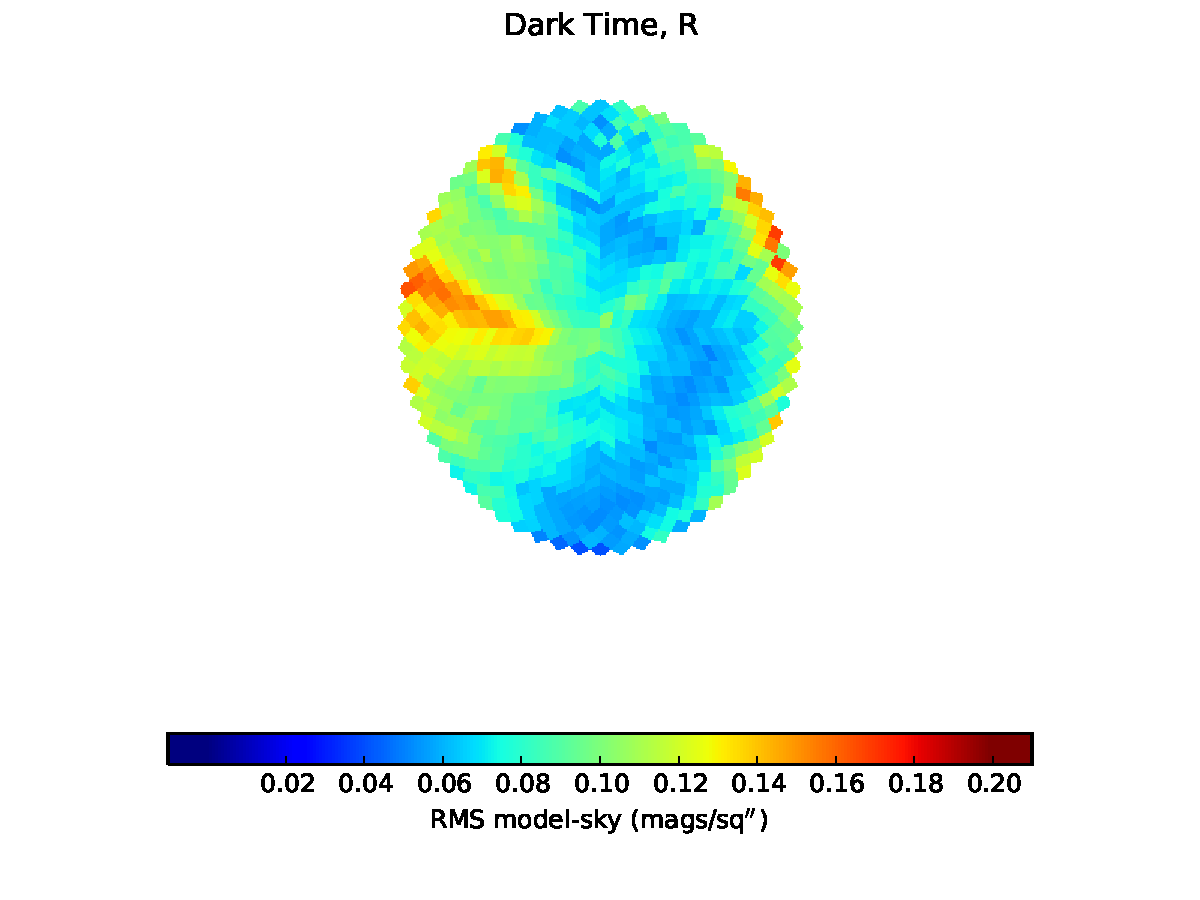
\includegraphics[height=5cm]{plots/stdResidMap_R.pdf}\includegraphics[height=5cm]{plots/stdResidMap_g.pdf}\includegraphics[height=5cm]{plots/stdResidMap_b.pdf}
  \end{center}
  \caption{Median and RMS maps of the model dark time residuals. The ``bright spot'' that is in the upper left of all the residual images could be scattered light }
\end{figure*}


Ref.~\citenum{Coughlin15} use the sun as a proxy for the moon to observe the expected lunar contribution to the night sky brightness in LSST filters. In Figure~\ref{fig:cCompare} we compare Figure~3 from Ref.~\citenum{Coughlin15} with the output of a night-time computation of our sky model.  The plots show $\Delta m_5$ as defined in Ref.~\citenum{Coughlin15} (basically, half the change in sky surface brightness in magnitudes).  

\begin{figure*}
  \begin{center}
  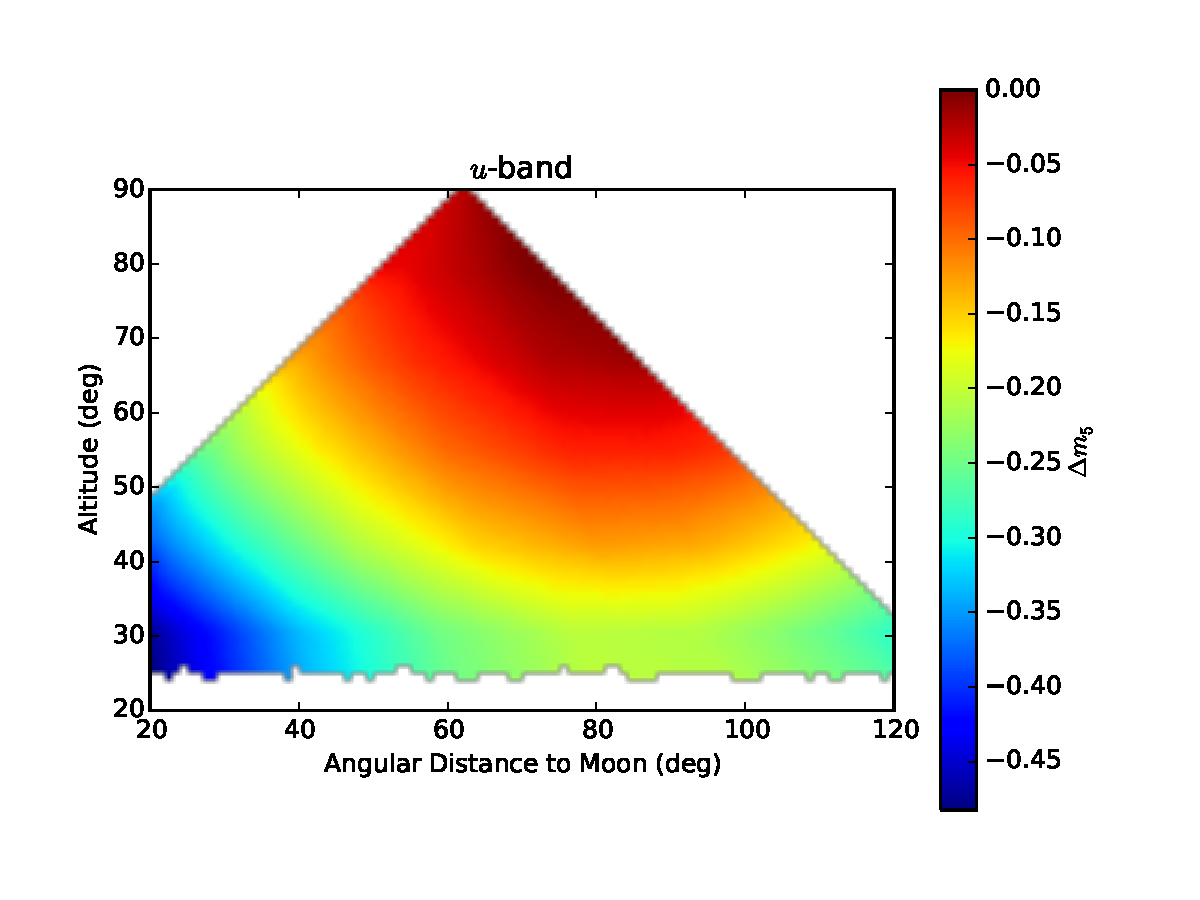
\includegraphics[height=5cm]{plots/deltam5.pdf}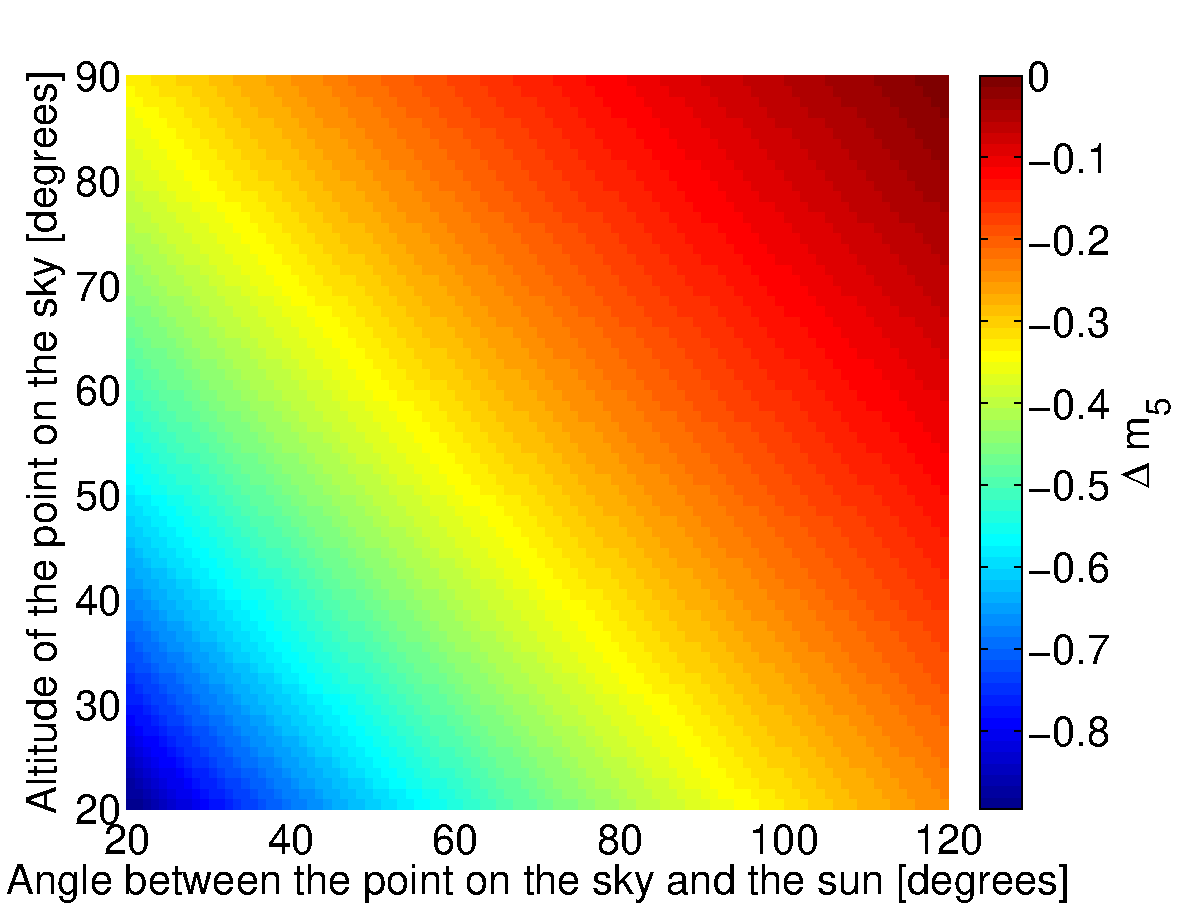
\includegraphics[height=5cm]{plots/a1_alt_angle_meshgrid.pdf}
  \end{center}
  \caption{ Comparison of our sky model (left) and observations of the sun by Ref.~\citenum{Coughlin15} (right).  We only calculate for a single time (when the moon is at an altitude of $\sim 30$ degrees. Unlike images taken when the sun is up, other emission components dominate at low altitude.  \label{fig:cCompare}}
\end{figure*}

\section{Conclusions}

As part of the LSST simulations software stack we have created a model for night sky emission.  In typical cloudless night time conditions, the model has a precision of $\pm$0.2-0.3 magnitudes arcsecond$^{-2}$. The model breaks down at airmasses higher than 2.5, near the moon (within $\sim15\degree$), and bright twilight (sun higher than -10$\degree$).  Unfortunately, because the underlying ESO code used to build our template library is not open-source, it is not possible to re-compute our template spectra library for observatories at very different altitudes.  

\acknowledgments        
 
We thank Tim Jenness and Michael Wood-Vasey for comments on a draft of this document.  This material is based upon work supported in part by the National Science Foundation through Cooperative Support Agreement (CSA) Award No. AST–1227061 under Governing Cooperative Agreement 1258333 managed by the Association of Universities for Research in Astronomy (AURA), and the Department of Energy under Contract No. DE–AC02–76SF00515 with the SLAC National Accelerator Laboratory. Additional LSST funding comes from private donations, grants to universities, and in-kind support from LSSTC Institutional Members.

\bibliography{skyModel}
\bibliographystyle{spiebib}

\end{document}

\section{Possible Future Work}

Note that we have not verified the off-zenith IR performance of the model. If the source of scattering of IR sunlight in the atmosphere is significantly different from optical light, the model could be wrong. Measuring the IR surface brightness of the twilight sky along just a few more alt-az pointings could help in verifying and constraining the $b$ and $c$ terms of Equation~\ref{eqn:twi}.

We have not included the sky brightness increase that can come from light reflected off of clouds.  With the data from the all-sky camera, we could construct a model for the increased brightness we expect as a function of atmospheric transparency.  

When fitting the all-sky twilight data, we assumed that as long as the moon had set we could approximate the sky background at a given airmass as constant. We should go back and remove the expected zodiacal light as well as airglow given the solar activity at the time of the observations. Thus, we should expect the the fits in Table~\ref{table:canonFits} to be slightly skewed by the presence of zodiacal light, particularly parameter $c$.  

When a spectrum is requested from the twilight model, we currently return a solar spectrum multiplied by a smooth spline curve to match the expected broad-band magnitudes.  While the twilight is solar-like, our simple procedure means the spectrum does not have the correct atmospheric absorption features.  A future improvement could be to use observed twilight spectra to make our returned results more realistic.

The sky model currently uses the pyEphem package to compute sun and moon positions as well as a few coordinate transformations. It would be preferable to eliminate this dependency.  

%%  LocalWords:  ESO SkyCalc airglow Noll numpy nm airmass Healpixel
%%  LocalWords:  nside Healpixels Krisciunas Patat twi az skyModel Gb
%%  LocalWords:  SIM Cerro Pachon photodiodes airmasses radians pre
%%  LocalWords:  photodiode zeropoint skybrightness stepsize Mauna
%%  LocalWords:  Kea Paranal brightnesses pointings SFU annulus NIST
%%  LocalWords:  radiative FORS healpix healpy pyEphem BVRI Gorski
%%  LocalWords:  Ivezic Coughlin
